\documentclass[english,11pt]{beamer}

\DeclareMathOperator{\Cov}{Cov}
\DeclareMathOperator{\Var}{Var}
\DeclareMathOperator{\E}{\mathbb{E}}
\DeclareMathOperator{\Proba}{\mathbb{P}}

\newcommand{\Covb}[2]{\ensuremath{\Cov\!\left[#1,#2\right]}}
\newcommand{\Eb}[1]{\ensuremath{\E\!\left[#1\right]}}
\newcommand{\Pb}[1]{\ensuremath{\Proba\!\left[#1\right]}}
\newcommand{\Varb}[1]{\ensuremath{\Var\!\left[#1\right]}}

% norm
\newcommand{\norm}[1]{\| #1 \|}

\newcommand{\indep}{\rotatebox[origin=c]{90}{$\models$}}





\usepackage{mathptmx,amsmath,amssymb,graphicx,bibentry,bbm,babel,ragged2e}

\makeatletter

\newcommand{\noun}[1]{\textsc{#1}}
\newcommand{\jitem}[1]{\item \begin{justify} #1 \end{justify} \vfill{}}
\newcommand{\sframe}[2]{\frame{\frametitle{#1} #2}}

\newenvironment{centercolumns}{\begin{columns}[c]}{\end{columns}}
%\newenvironment{jitem}{\begin{justify}\begin{itemize}}{\end{itemize}\end{justify}}

\usetheme{Warsaw}
\setbeamertemplate{footline}[text line]{}
\setbeamercolor{structure}{fg=purple!50!blue, bg=purple!50!blue}

\setbeamersize{text margin left=15pt,text margin right=15pt}

\setbeamercovered{transparent}


\@ifundefined{showcaptionsetup}{}{%
 \PassOptionsToPackage{caption=false}{subfig}}
\usepackage{subfig}

\usepackage[utf8]{inputenc}
\usepackage[T1]{fontenc}



\makeatother

\begin{document}


\title{Co-construire Modèles, Etudes Empiriques et Théories en Géographie Théorique et Quantitative : le cas des Interactions entre Réseaux et Territoires}

\author{J.~Raimbault$^{1,2}$\\
\texttt{juste.raimbault@parisgeo.cnrs.fr}
}


\institute{$^{1}$UMR CNRS 8504 G{\'e}ographie-cit{\'e}s\\
$^{2}$UMR-T IFSTTAR 9403 LVMT\\
}


\date{13èmes Rencontres Théo Quant - Besançon\\\smallskip
Atelier 1 : Modélisation et Simulation Urbaine (1)\\\smallskip
17 mai 2017
}

\frame{\maketitle}





%%%%%%%%%%%%%%%%%%%
%% ABSTRACT
%\textbf{Mots-clés : } Co-construction des Connaissances ; Méthodologie de la Géographie Théorique et Quantitative ; Interaction entre Réseaux et Territoires





%%%%%%%%%%%%%%%%%
\section{Introduction}
%%%%%%%%%%%%%%%%%


%La construction de théories géographiques, dans le cadre d'une Géographie Théorique et Quantitative, s'effectue par itérations dans une dynamique de co-évolution avec les efforts empiriques et de modélisation~\cite{livet2010}. Parmi les nombreux exemples, on peut citer la théorie évolutive des villes (co-construite par un spectre de travaux s'étendant par exemple des premières propositions de \cite{pumain1997pour} jusqu'aux résultats matures présentés dans~\cite{pumain2012multi}), l'étude du caractère fractal des structures urbaines (par exemple de \cite{frankhauser1998fractal} à \cite{frankhauser2008fractal}) ou plus récemment le projet Transmondyn visant à enrichir la notion de transition des systèmes de peuplement (ouvrage à paraître). Cette communication propose un format original en s'inscrivant dans cette lignée, par la synthèse de différents travaux empiriques et de modélisation menés conjointement avec l'élaboration d'appareils théoriques visant à mieux comprendre les relations entre territoires et réseaux de transports. L'originalité de cette contribution réside à la fois dans la synthèse de travaux très divers pourtant reliés en filigrane, et dans la proposition d'une théorie géographique spécifique s'appuyant sur cette synthèse en seconde partie.

%%%
%  Accroche ?
%   - contexte TQG : Cuyala, Pumain-Robic
%   - domaines de connaissance : classiques ? (cit. étendu seulement, en slide annexe)
\sframe{TQG et Domaines de Connaissance}{

\justify

Le Meilleur endroit pour parler de Géographie Théorique et Quantitative ? \textit{Un an sur deux avec ECQTG !}

\bigskip

Quelle identité pour la TQG ? Nouvelles méthodes et outils\\
\cite{pumain2002role} ; une particularité Européenne \cite{cuyala2013diffusion}. Existence cependant avérée d'épistémologies propres cohérentes (pour déplaire à \cite{ripoll2017jig})

\bigskip

\textbf{Postulat : } \textit{L'essence de la TQG est dans le couplage fort et la co-construction des domaines de connaissances - initialement Théorie, Modélisation et Empirique au sens de \cite{livet2010} ; extension aux Méthodes, Outils et Données par \cite{raimbault:halshs-01505084} décrivant un cadre épistémologique pour une Géographie Intégrée.}

%\textbf{{\fontencoding{U}\fontfamily{futs}\selectfont\char 66\relax}} Enfoncer des portes ouvertes ? \textit{Si personne n'y rentre sont-elles vraiment ouvertes ? cf. \cite{legavre1996neutralite}}
}

\sframe{Illustrations}{
%   - example frankhauser, Transmondyn

Exemples de théories de référence illustrant cette co-construction :

\bigskip

$\rightarrow$ Théorie fractale des structures urbaines. De \cite{frankhauser1998fractal} à \cite{frankhauser2008fractal} : théorie, études de cas, données, méthodes (estimateurs, morpho. math.), outils (fractalyse)

\medskip

$\rightarrow$ Projet TransmoDyn et transitions des systèmes de peuplements : co-construction renforcée par l'intégration disciplinaire

\medskip

$\rightarrow$ Théorie Evolutive des Villes

}


\sframe{Théorie Evolutive des Villes}{
%   - analyse interviews de la Th. Evolutive

% Application : 
% Lecture de la théorie évolutive au regard de ce fwk (différent application concrète)

% broad view of the importance of knowledge co-evolution in evolutive urban theory
% try to give a sketch of what is it ?

% org des villes dans territoires
%ambition : rassembler essentiel faits stylisés, les placer pas dasn une th disciplinaire, ou equilibre, structure statiques, mais perspectives spatio temporels qui permet de les suivre sur longues periodes de temps ; attention aux principaux facteurs structurants : systèmes ; attention à observer bifurcation ; en ce sens, systèmes complexes pour aider : villes dans des systèmes de ville, Berry considérablement revisité ; ville objet complexe pas indépendant, inséré dans ses réseaux ; mieux 

\vspace{-0.8cm}

\justify

{\footnotesize
\textbf{Définition : }\textit{Une Théorie Géographique ayant pour ambition de rassembler la plupart des faits stylisés connus sur les villes et leur organisation dans les territoires, dans une perspective hors-équilibre et non statique, en les suivant sur de longues périodes de temps et mettant une emphase sur les facteurs structurants et les bifurcations.} [Entretien avec D. Pumain, 03/2017]
}

\small

\smallskip

$\rightarrow$ Travaux précurseurs : manifeste théorique \cite{pumain1997pour} et modélisation \cite{sanders1997simpop} 

\smallskip

$\rightarrow$ Relations ``gagnant-gagnant'' avec les informaticiens [Entretien avec R. Reuillon, 04/2017] : OpenMole \cite{reuillon2013openmole} et Meta-heuristiques \cite{10.1371/journal.pone.0138212} 

\smallskip
%

$\rightarrow$ Terrains variés et poussés (\cite{swerts2013systemes} \cite{baffi:tel-01389347}), modélisations intégrées (\cite{cottineau2014evolution} \cite{schmitt2014modelisation}), épistémologie \cite{rey2015plateformeshort} 

\smallskip

$\rightarrow$ Cadre théorique et méthodes pou renouveler les ontologies : ex. def. ville [Entretien avec C. Cottineau, 05/2017]

\smallskip

$\rightarrow$ L'analyse quantitative (réseau de citation) confirme cette structure (en revue)

}

%\sframe{Théorie Evolutive des Villes}{
%   - analyse network de la th. evolutive
%  Also do not include, under review
%}


\sframe{Contexte et Démarche}{
%   - slide "biblio" sur modelisation networks and territories : pourquoi on s'y interesse
%   - puis explication de la démarche (évoquer co-evol des domaines)

\textit{Une illustration sur un exemple ``vivant''}

\bigskip

\textbf{Objet d'étude : } Interactions entre réseaux de transports et territoires. Débats récurrents sur des causalités circulaires complexes~\cite{offner1993effets} ; Existence d'une co-évolution \cite{bretagnolle:tel-00459720} mais peu de modèles l'endogénéisant

\bigskip

$\rightarrow$ Synthèse de travaux en cours visant à construire des modèles de co-évolution : mobilise les différents domaines et implique une construction théorique.

\medskip

% mentionner ouvrage qui prend la poussière dans une étagère ; pas de rapport avec exo de synthèse et d'écriture, on peut très bien faire synthèse ET écriture via media alternatifs

\textbf{{\fontencoding{U}\fontfamily{futs}\selectfont\char 66\relax}} Difficulté de la narration linéaire : modèles de communication à renouveler impérativement ? (pauvreté de la lecture linéaire, mémoires prenant la poussière dans l'étagère \ldots )

}







%%%%%%%%%%%%%%%%%
\section{Etudes de cas et Modèles}
%%%%%%%%%%%%%%%%%



%\paragraph{Pourquoi une théorie et des modèles de co-évolution}
%Notre première entrée prend un point de vue d'épistémologie quantitative pour tenter d'expliquer le fait que, si la co-évolution entre territoires et réseaux a par exemple été prouvée par~\cite{bretagnolle:tel-00459720}, la littérature est très pauvre en modèles de simulation endogénéisant cette co-évolution. Une exploration algorithmique de la littérature a été menée dans \cite{raimbault2015models}, suggérant un cloisonnement des domaines scientifiques s'intéressant à ce sujet. Des méthodes plus élaborées ainsi que les outils correspondants (collecte et analyse des données), couplant une analyse sémantique au réseau de citations, ont été développées pour renforcer ces conclusions préliminaires~\cite{raimbault2016indirect}, et les premiers résultats au second ordre semblent confirmer l'hypothèse d'un domaine peu défriché car à l'intersection de champs ne dialoguant pas nécessairement aisément. Ces premiers résultats d'épistémologie quantitative confirment l'intérêt d'une modélisation couplant des processus relevant de différentes échelles et domaines d'études, et surtout l'intérêt de l'élaboration d'une théorie propre.

\sframe{Pourquoi une théorie et des modèles de co-évolution}{
% epistemo quanti

\vspace{-0.5cm}
{\footnotesize \justify
\cite{raimbault2015models} : Revue Systématique Algorithmique reconstruisant la structure sémantique des disciplines étudiant un sujet donné ; Extension des méthodes et outils à une approche par hyperréseau dans \cite{raimbault2016indirect}
% ; Application à un corpus d'un autre type (brevets) \cite{bergeaud2017classifying} : nouvelle façon d'étudier empiriquement la diffusion spatiale des innovations ? (validation de la Théorie Evolutive urbaine)

$\rightarrow$ \textit{cloisonnement disciplinaire fort : objet intermédiaire peu étudié par des disciplines ne communiquant pas, d'où l'intérêt de modèle et d'une théorie propre.}

}

\centering
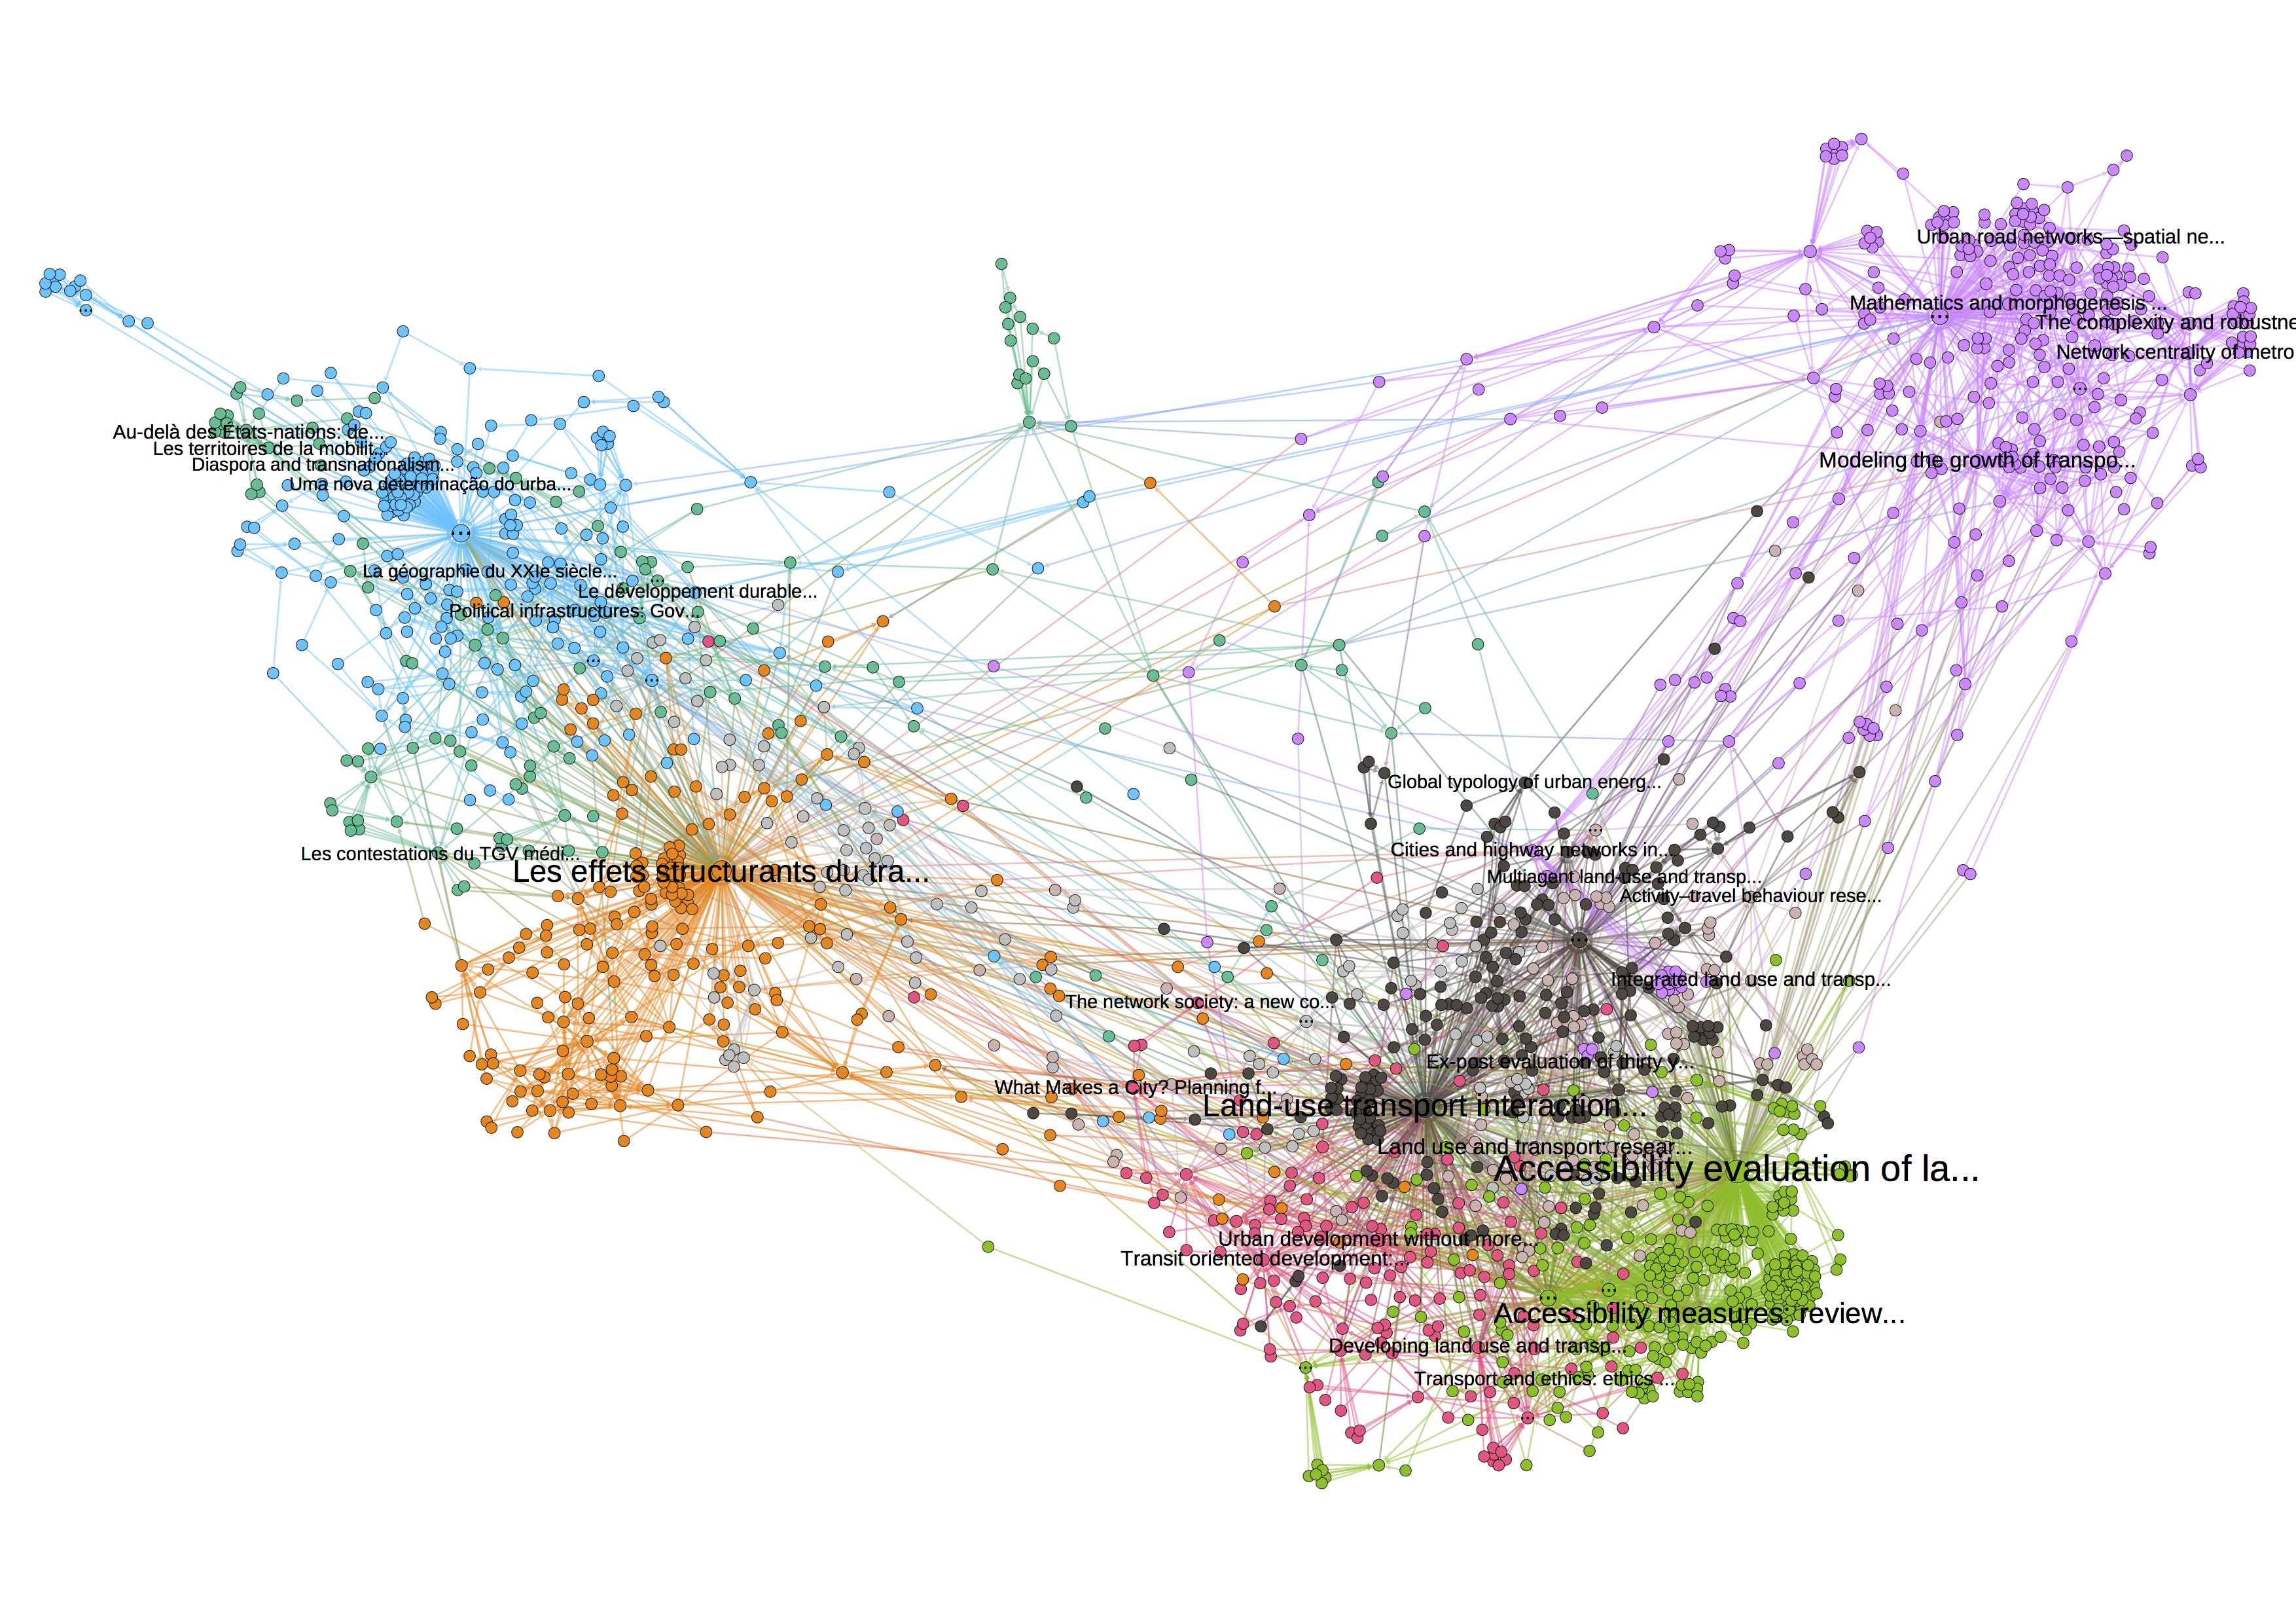
\includegraphics[width=0.6\textwidth]{figures/biblio_rawcore}
%\includegraphics[width=0.48\textwidth]{figures/cyb_semantic}
\hspace{0.3cm}
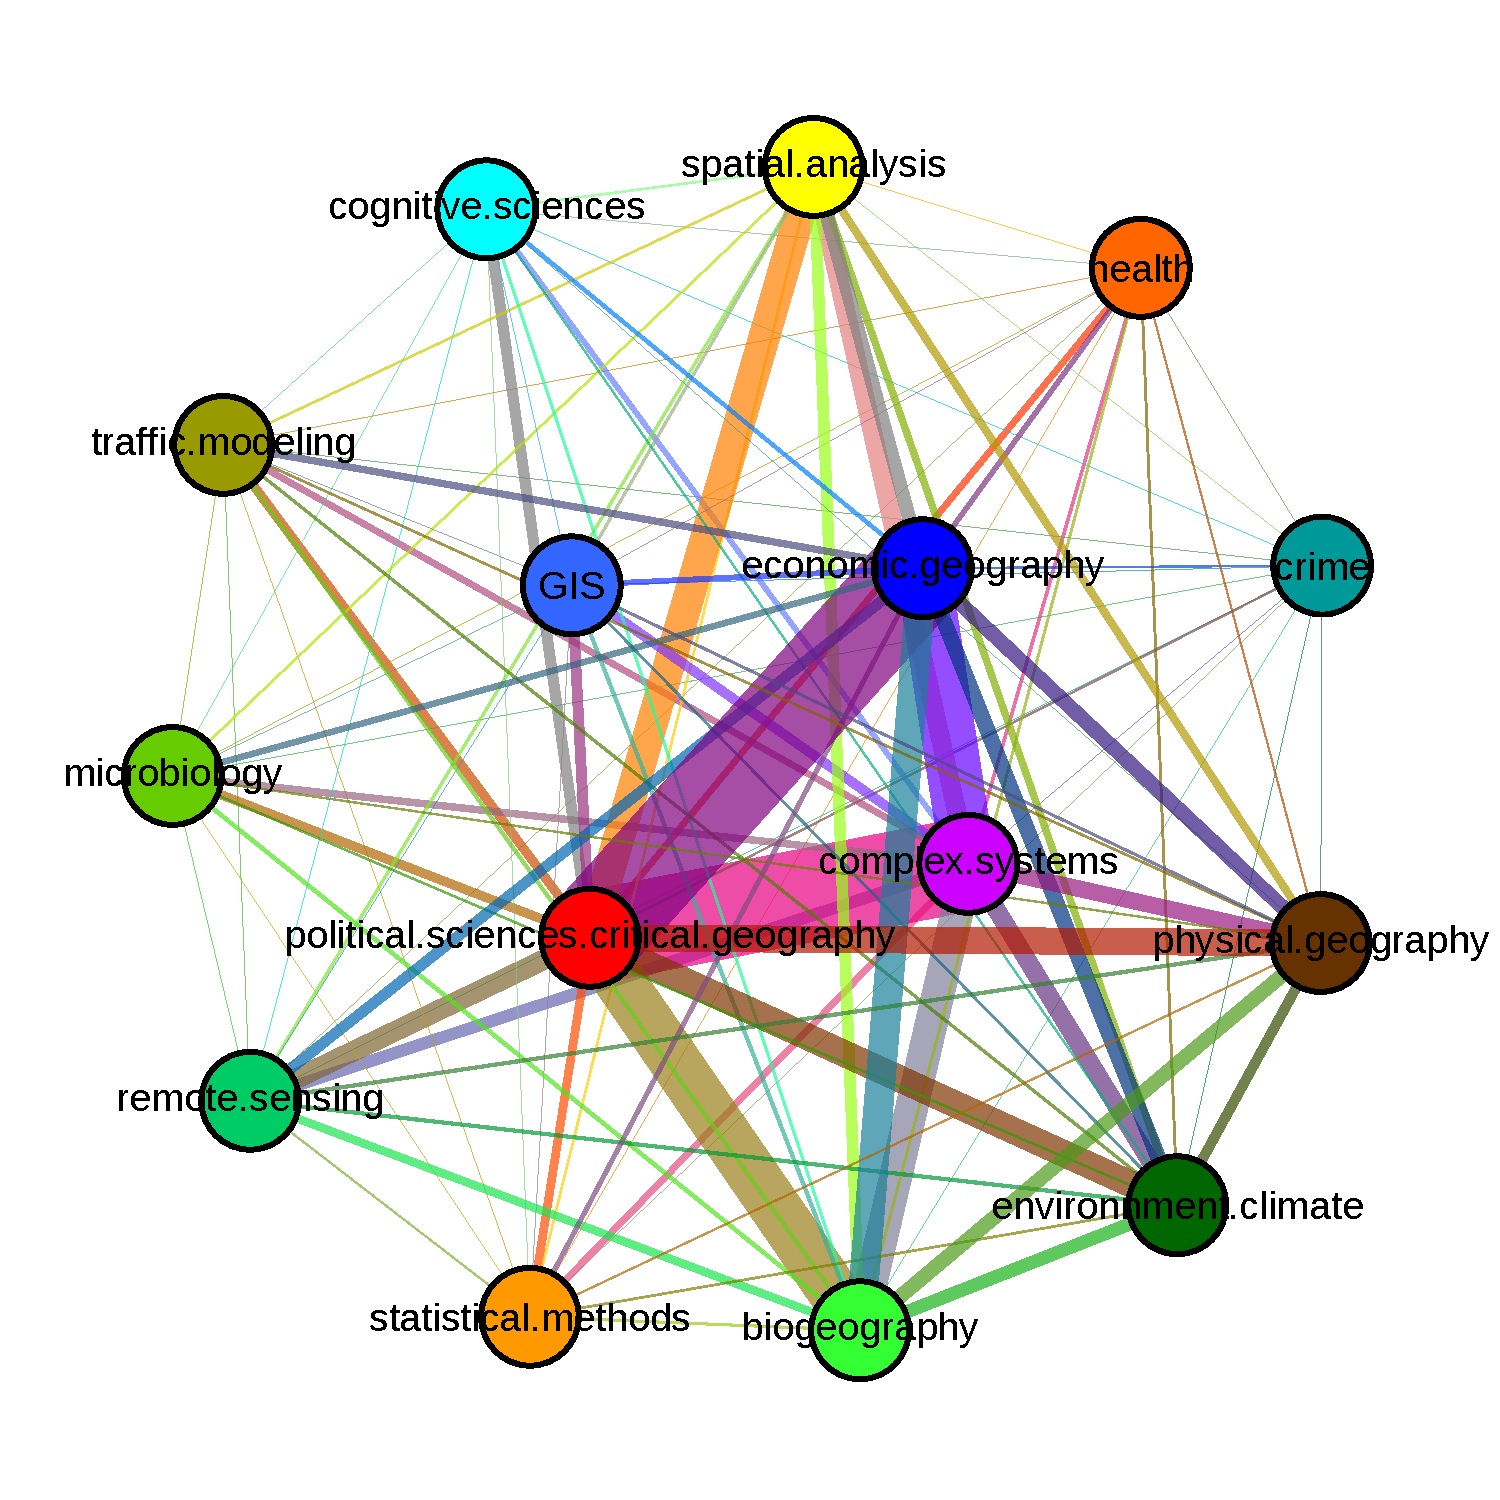
\includegraphics[width=0.3\textwidth]{figures/cyb_synththemcyb}

\footnotesize

\textit{(Gauche) Réseau de citations fortement modulaire ; (Droite) illustration de la reconstruction sémantique de disciplines}

}





%\paragraph{Etudes empiriques}
%Le premier axe pour les développements en eux-mêmes consiste en des analyses empiriques. Une étude des corrélations spatiales statiques entre mesures de forme urbaine (indicateurs morphologiques calculés sur la grille de population eurostat) et mesures de forme de réseau (topologie du réseau routier issu d'OpenStreetMap), sur l'ensemble de l'Europe à différentes échelles, a pu révéler la non-stationnarité et la multi-scalarité spatiale de leurs interactions~\cite{raimbault2016cautious}. Cet aspect a aussi été mis en évidence dans l'espace et le temps à une échelle microscopique lors de l'étude des dynamiques d'un système de transport~\cite{raimbault2016investigating}, conjointement avec l'hétérogénéité des processus pour un autre type de système~\cite{raimbault2015hybrid}. Ces faits stylisés valident pour l'instant l'utilisation de modèles de simulation complexes, pour lesquels des premiers efforts de modélisation ont ouvert la voie vers des modèles plus élaborés.

\sframe{Dynamiques Chaotiques des Systèmes de Transport}{

\small
\justify

\vspace{-0.4cm}

Etude de l'existence empirique de l'Equilibre Utilisateur Statique sur le réseau autoroutier d'Ile-de-France~\cite{raimbault2017investigating}

$\rightarrow$ \textit{Non-stationnarité et caractère chaotique des dynamiques à l'échelle microscopique}

\medskip

\begin{columns}
\column{0.45\textwidth}
\centering
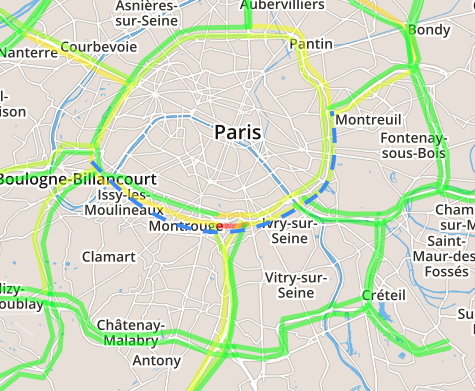
\includegraphics[width=0.65\textwidth]{figures/treq_gr21}\\\medskip
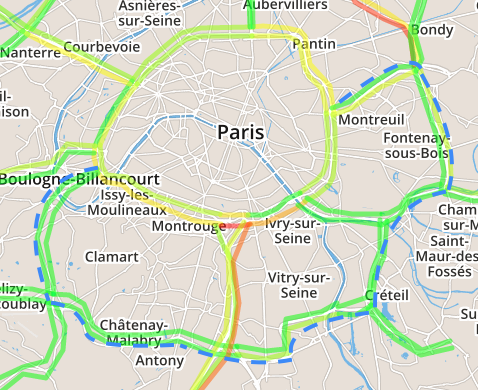
\includegraphics[width=0.65\textwidth]{figures/treq_gr22}

\column{0.55\textwidth}
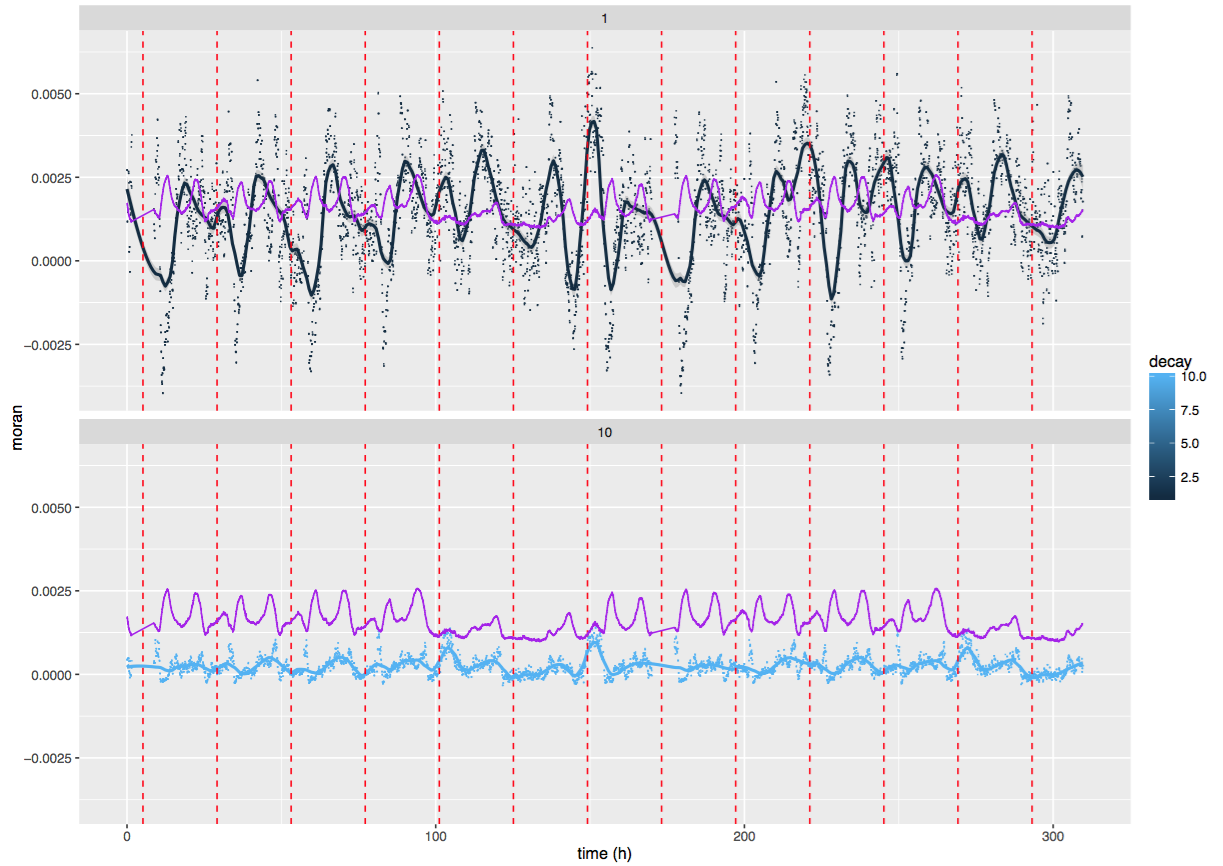
\includegraphics[width=\textwidth]{figures/treq_gr5}

\end{columns}

}

\sframe{Modélisation Basée-agent d'un Système de Transport}{

\small

Un modèle agent pour tester des interventions basées sur l'utilisateur pour un système de vélo en partage \cite{raimbault2015user} ; modélisation hybride avec statistiques et choix discrets \cite{raimbault2015hybrid}

\bigskip

$\rightarrow$ \textit{Nécessité d'une prise en compte de l'hétérogénéité des processus}

\bigskip

\begin{columns}
\column{0.55\textwidth}
\centering
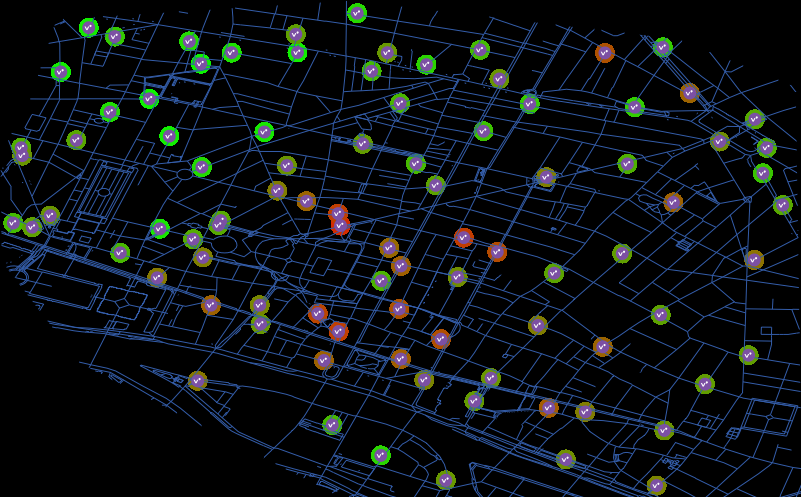
\includegraphics[width=0.9\textwidth]{figures/bikesharing_lfMidday}

\column{0.45\textwidth}
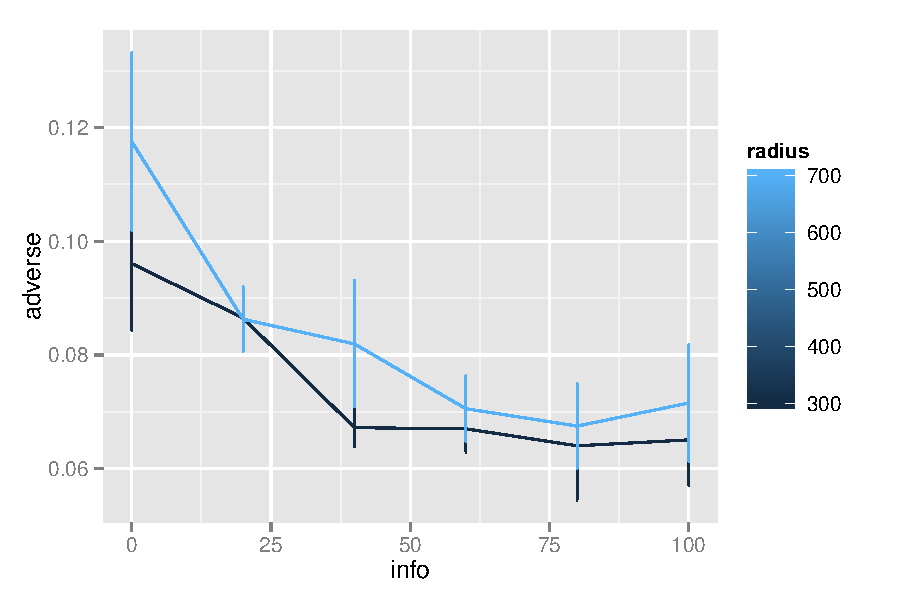
\includegraphics[width=\textwidth]{figures/bikesharing_adverse}

\end{columns}

}


% Q : what does it bring ? find a shitty link. multi-scalar ?
\sframe{Analyse des Réseaux Routiers}{

\vspace{-0.2cm}

Etude systématique de la topologie des réseaux routiers européens, corrélation des indicateurs avec leur résilience

$\rightarrow$ \textit{Variabilité spatiale et caractère multi-scalaire des processus}

\smallskip

\begin{columns}
\column{0.26\textwidth}
\centering
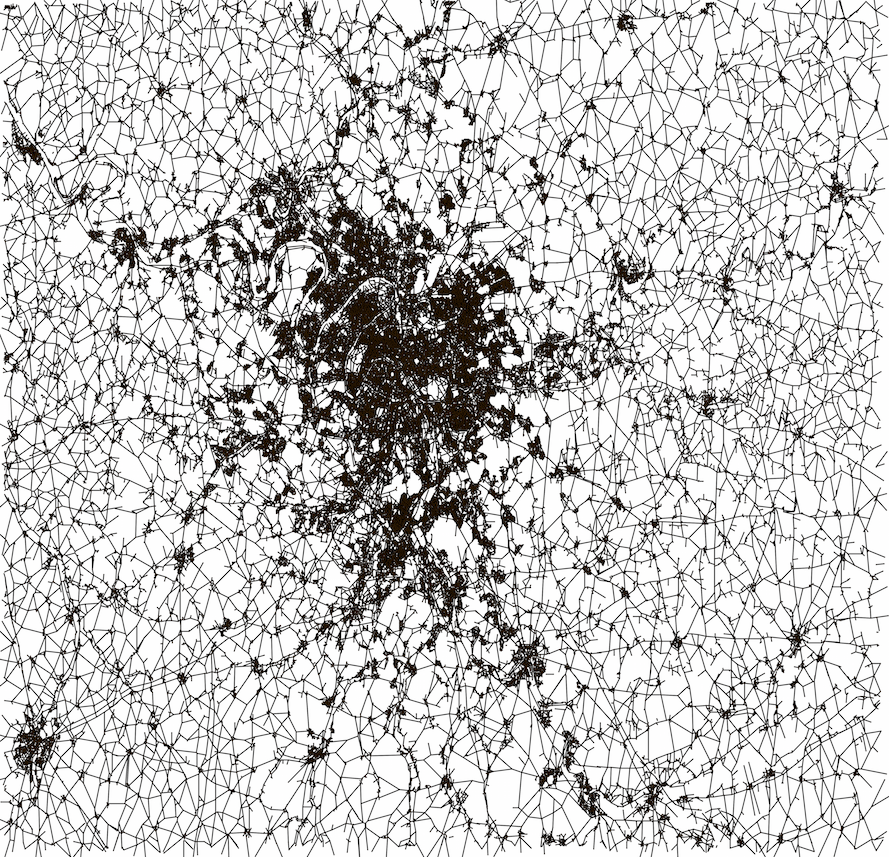
\includegraphics[width=\textwidth]{figures/nwanal_idf_lowres.png}\\
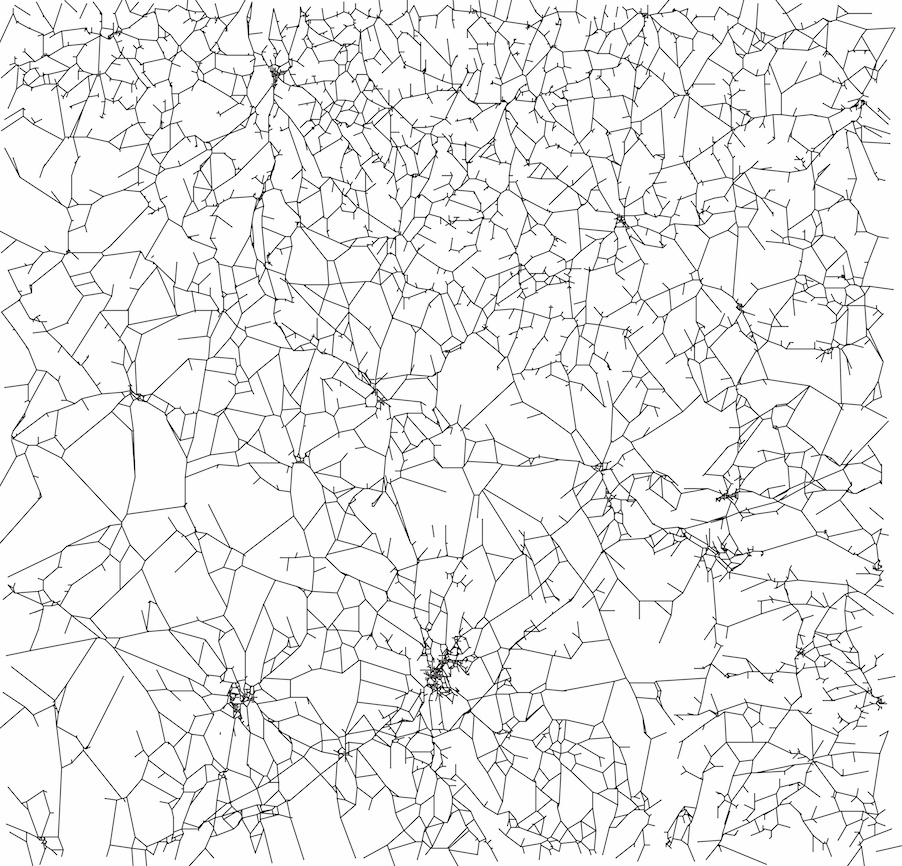
\includegraphics[width=\textwidth]{figures/nwanal_lacourtine_lowres.png}
\column{0.25\textwidth}
\centering
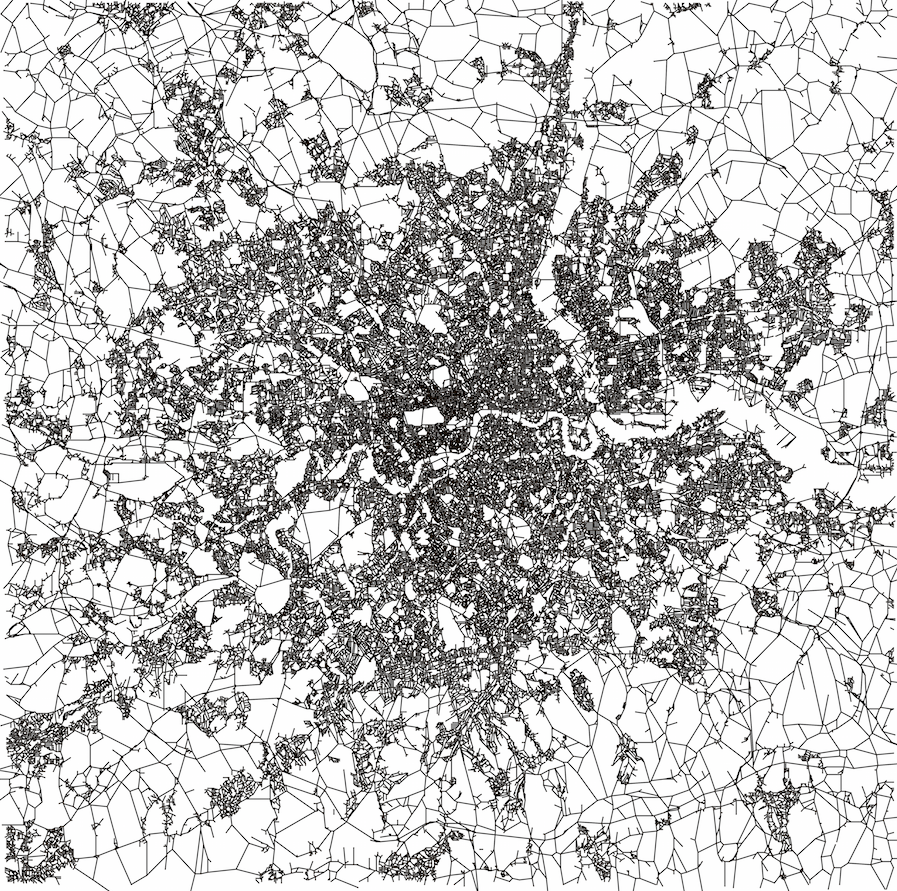
\includegraphics[width=\textwidth]{figures/nwanal_londonM25_lowres.png}\\
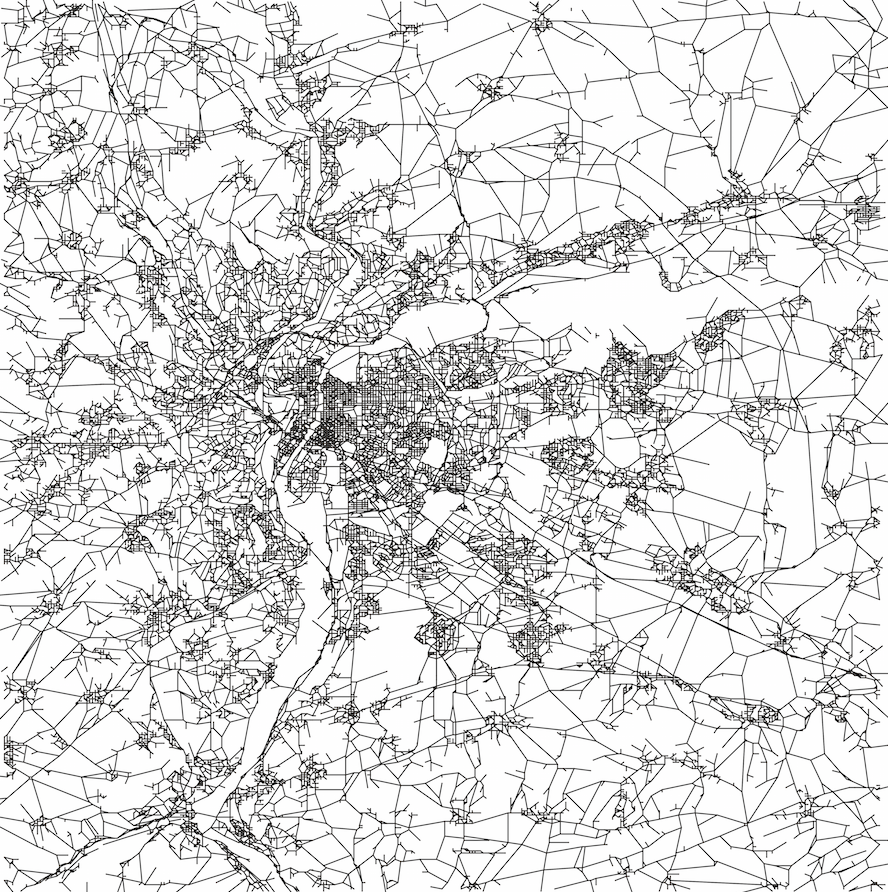
\includegraphics[width=\textwidth]{figures/nwanal_lyon_lowres.png}
\column{0.24\textwidth}
\centering
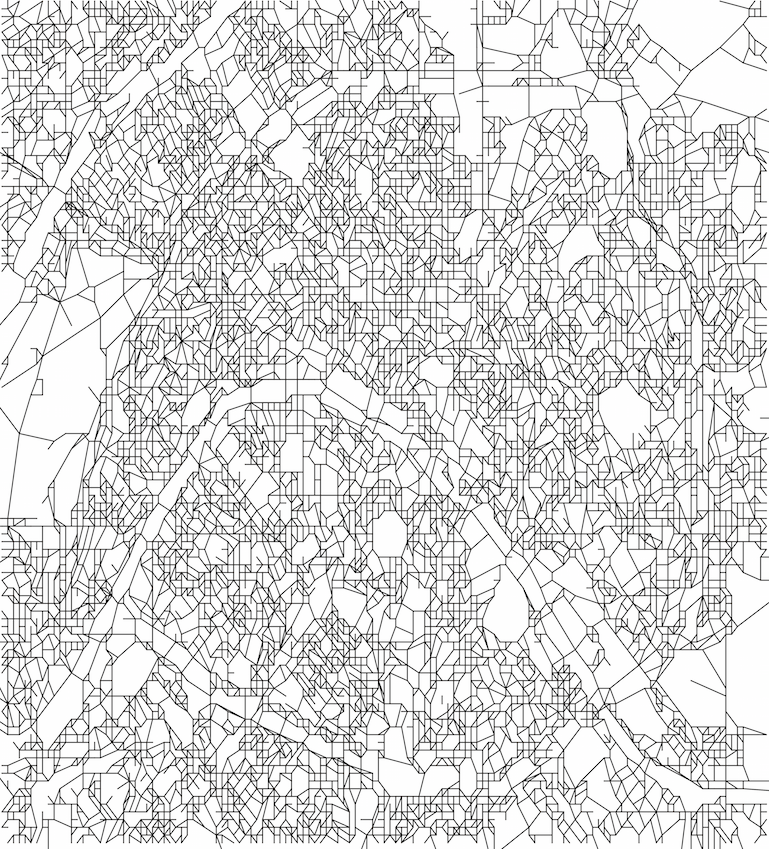
\includegraphics[width=\textwidth]{figures/nwanal_paris_lowres.png}\\
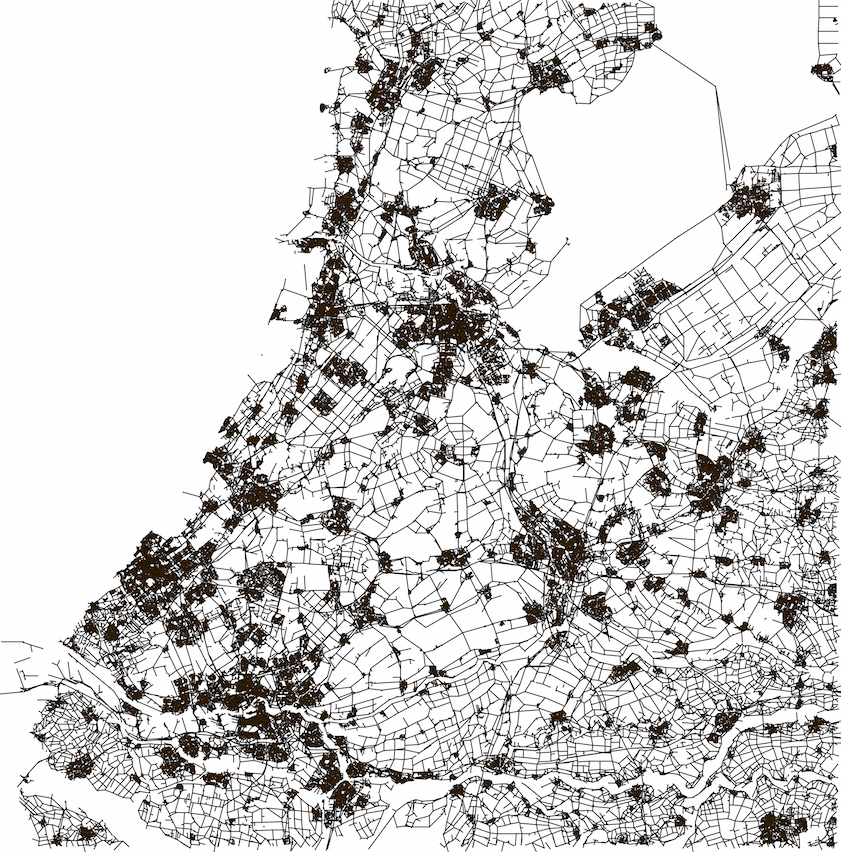
\includegraphics[width=\textwidth]{figures/nwanal_randstad_lowres.png}
\column{0.25\textwidth}
\centering
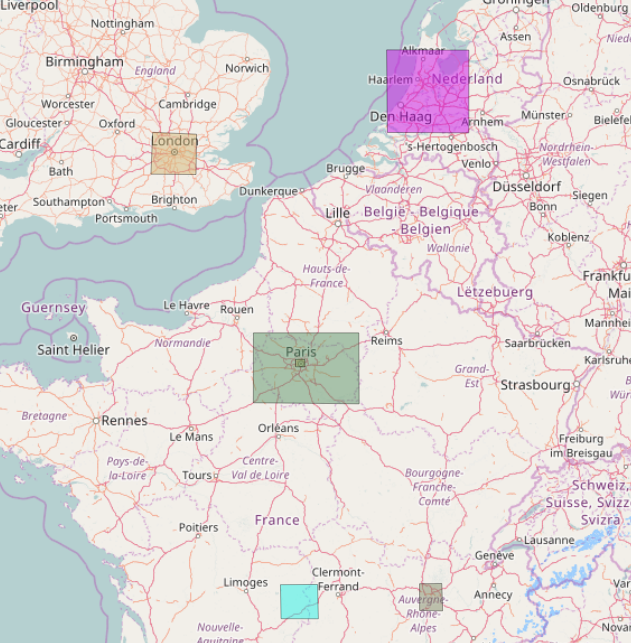
\includegraphics[width=\textwidth]{figures/nwanal_areas.png}

\end{columns}
}




%
\sframe{Correlations spatiales}{

\justify

\cite{raimbault2016cautious} : Données, outils et méthodes montrant la non-stationnarité spatiale et multi-scalarité des correlations entre forme urbaine et topologie des réseaux




\begin{columns}
\column{0.4\textwidth}\centering
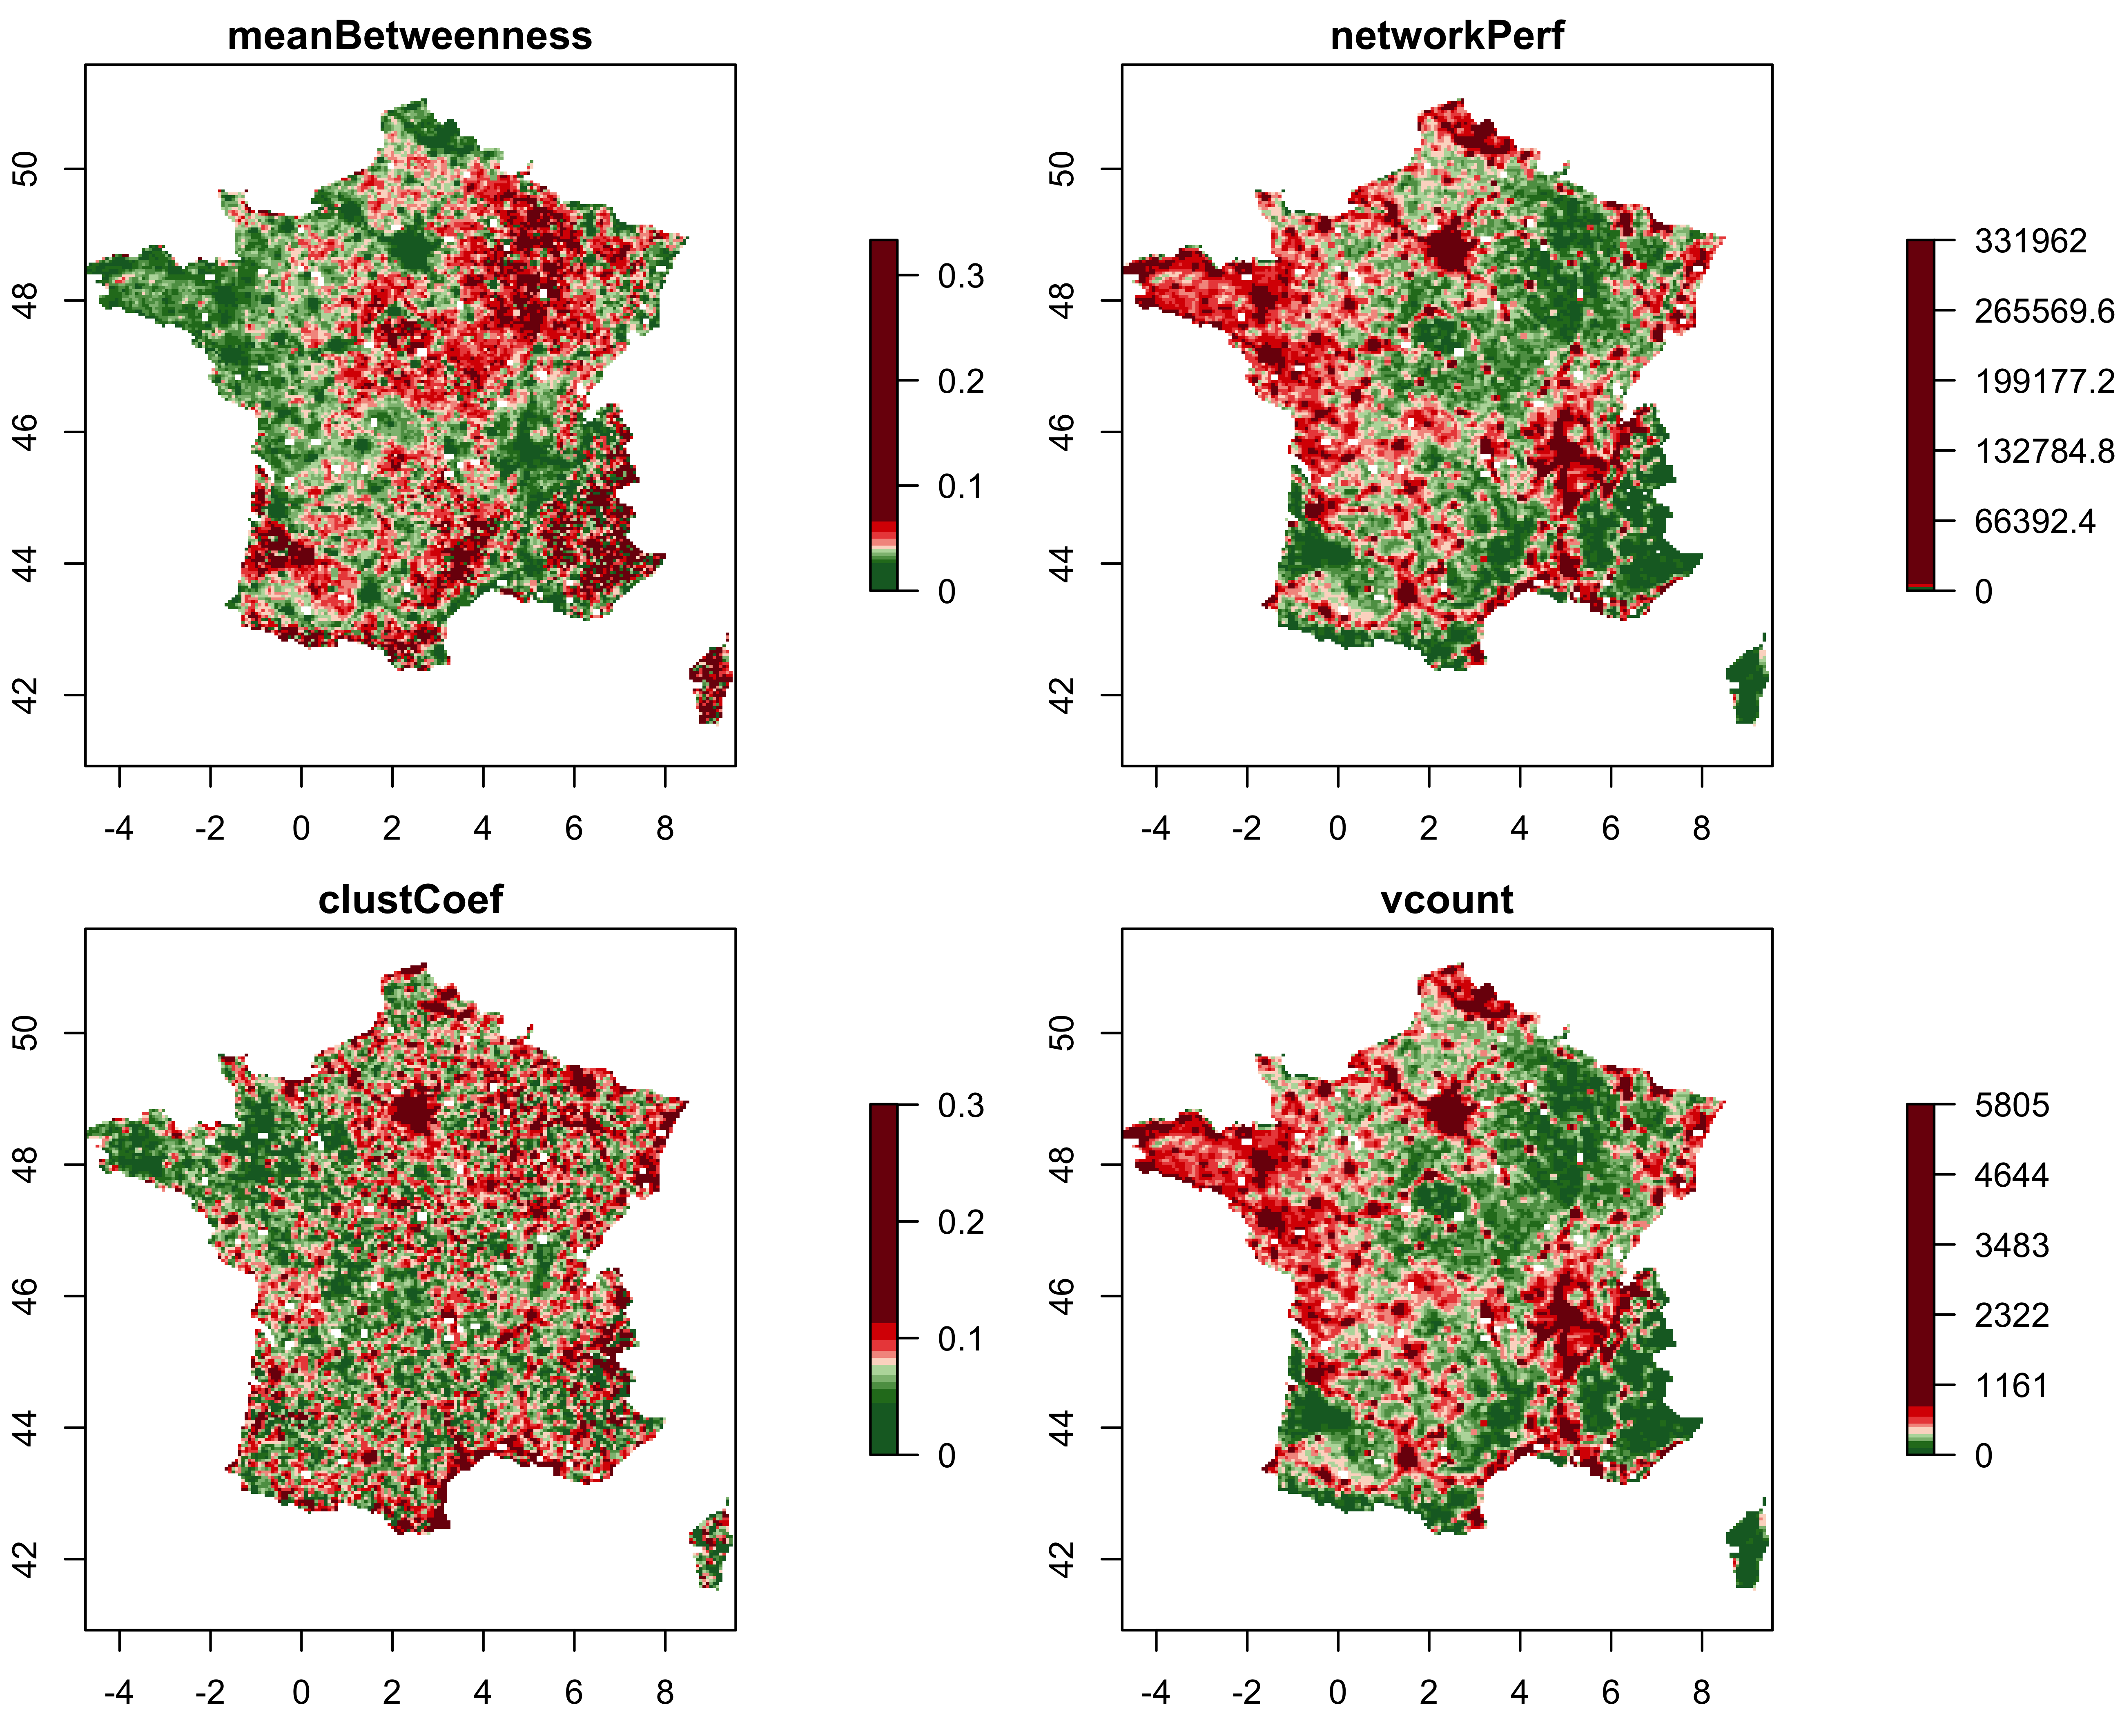
\includegraphics[width=\textwidth]{figures/morpho_indics_network_selected_discrquantiles.png}

\column{0.3\textwidth}\centering
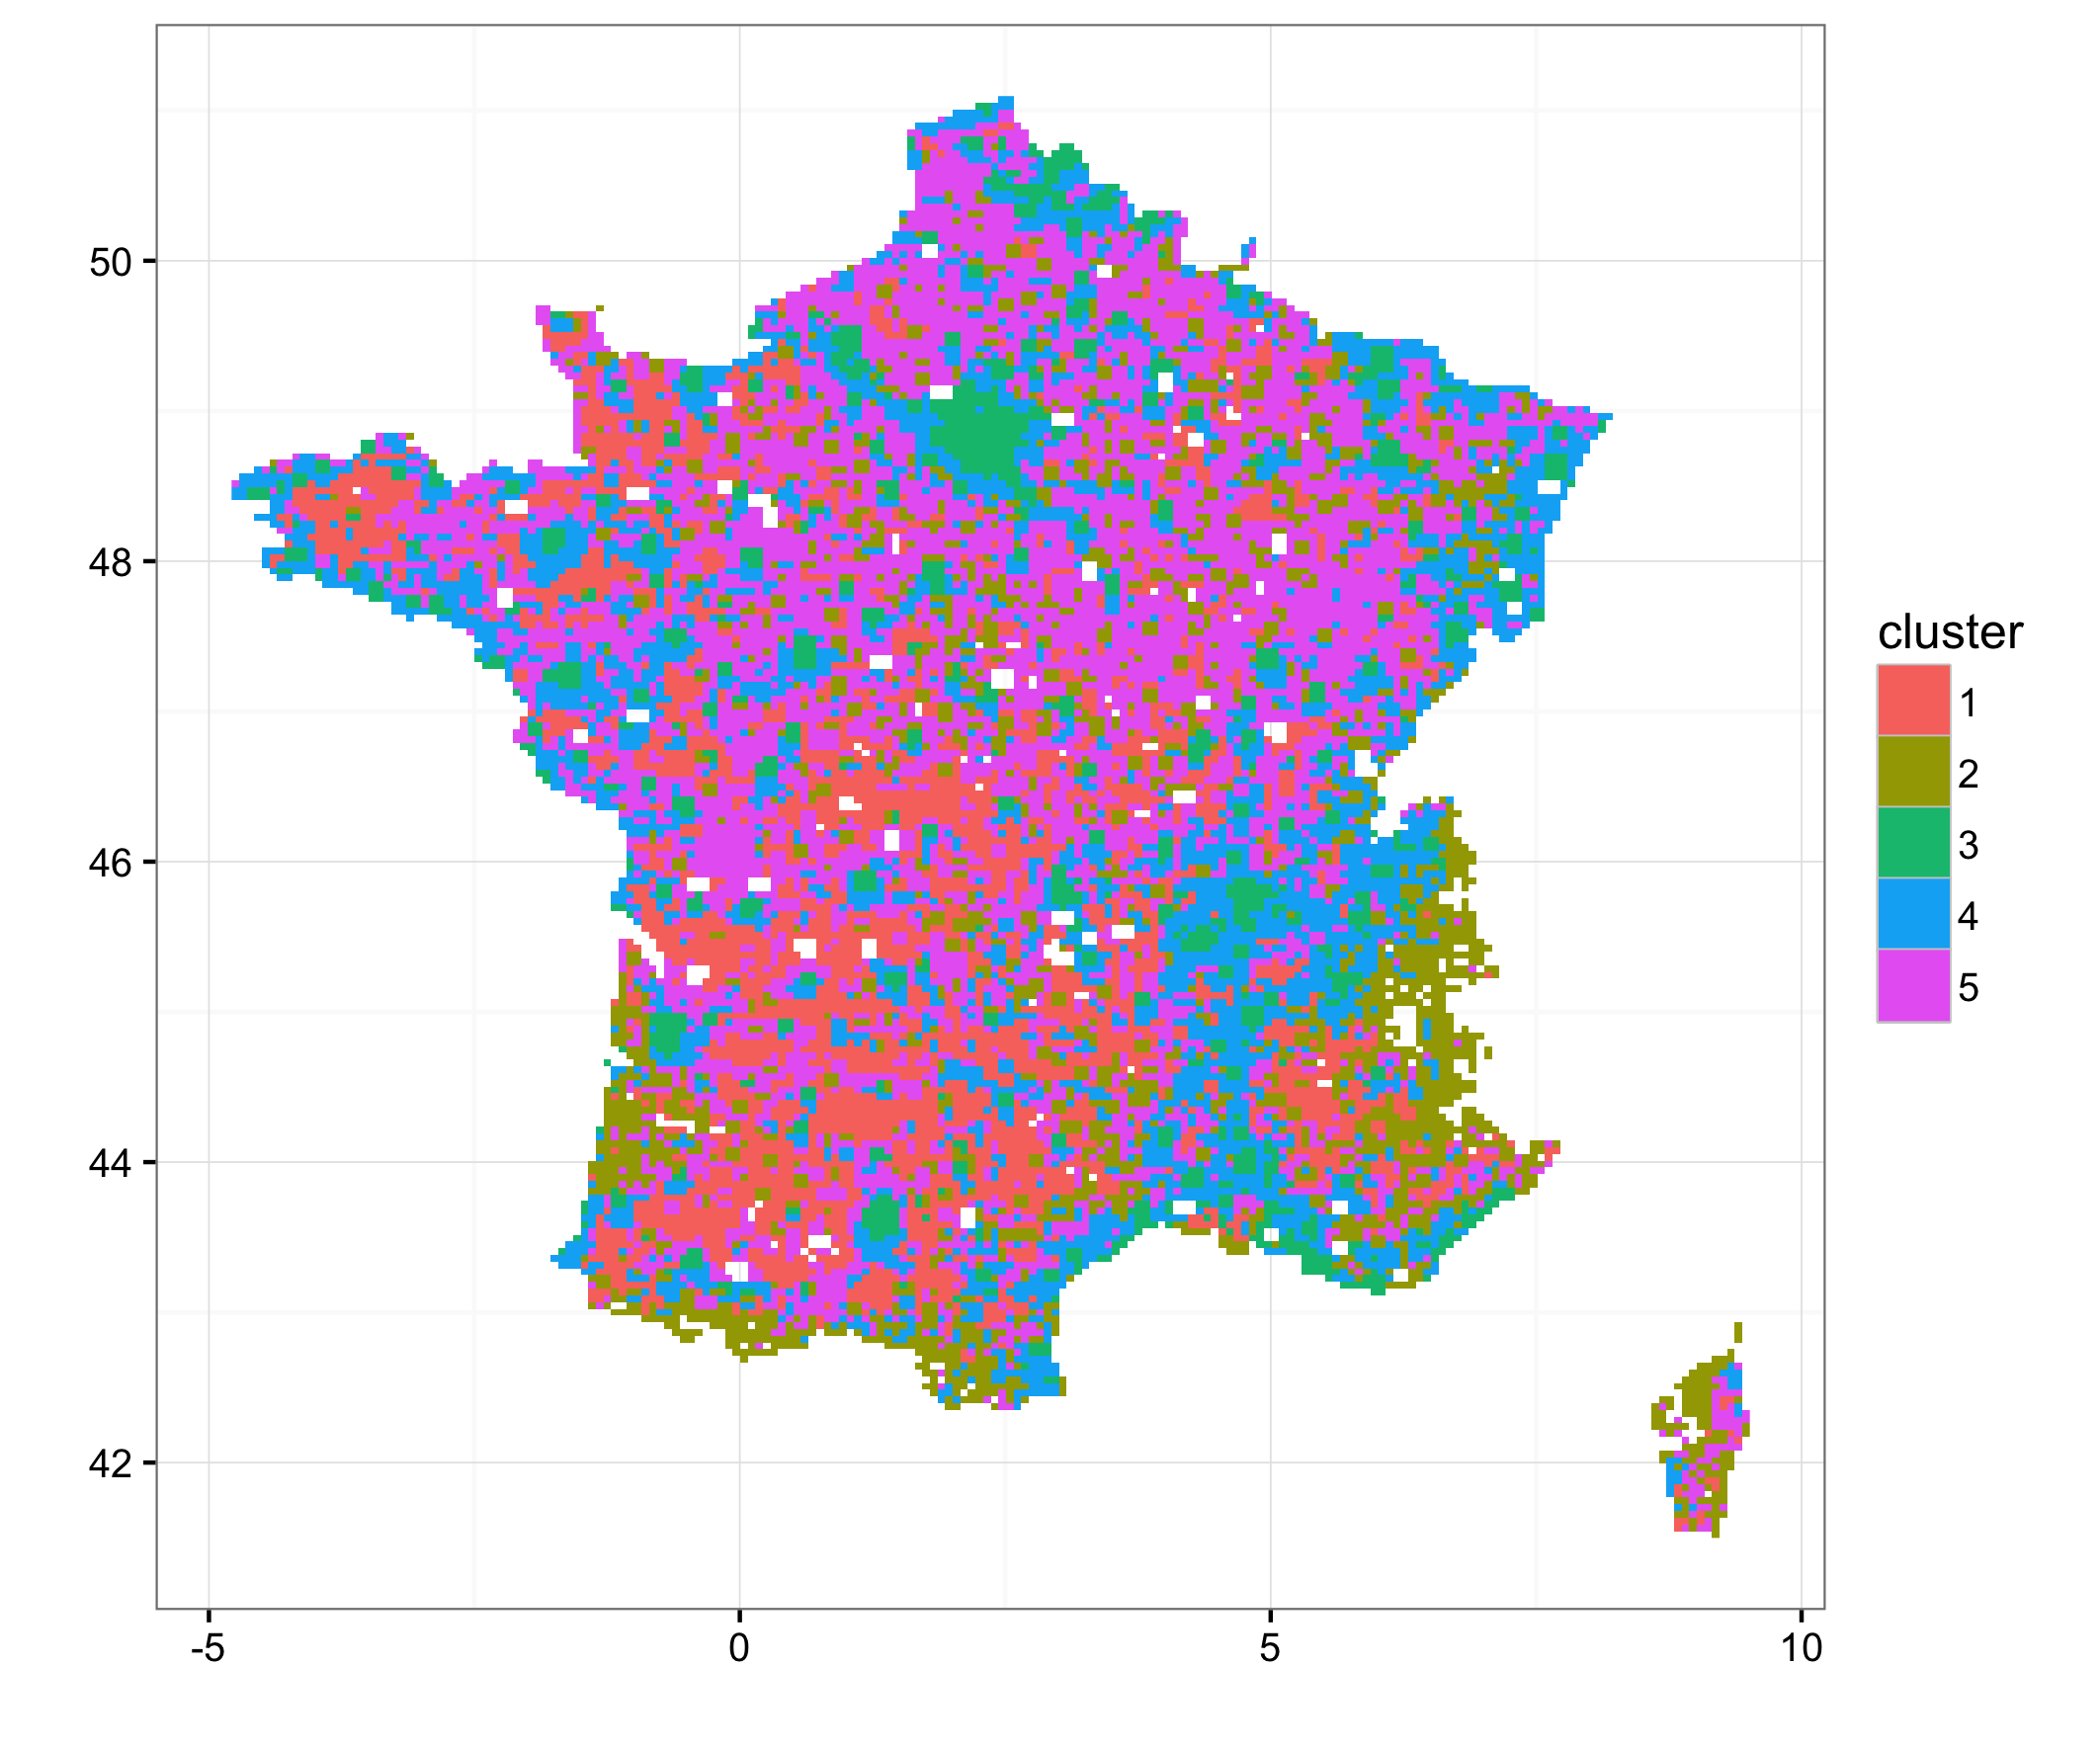
\includegraphics[width=\textwidth]{figures/morpho_cluster_map_k5_full.png}\\
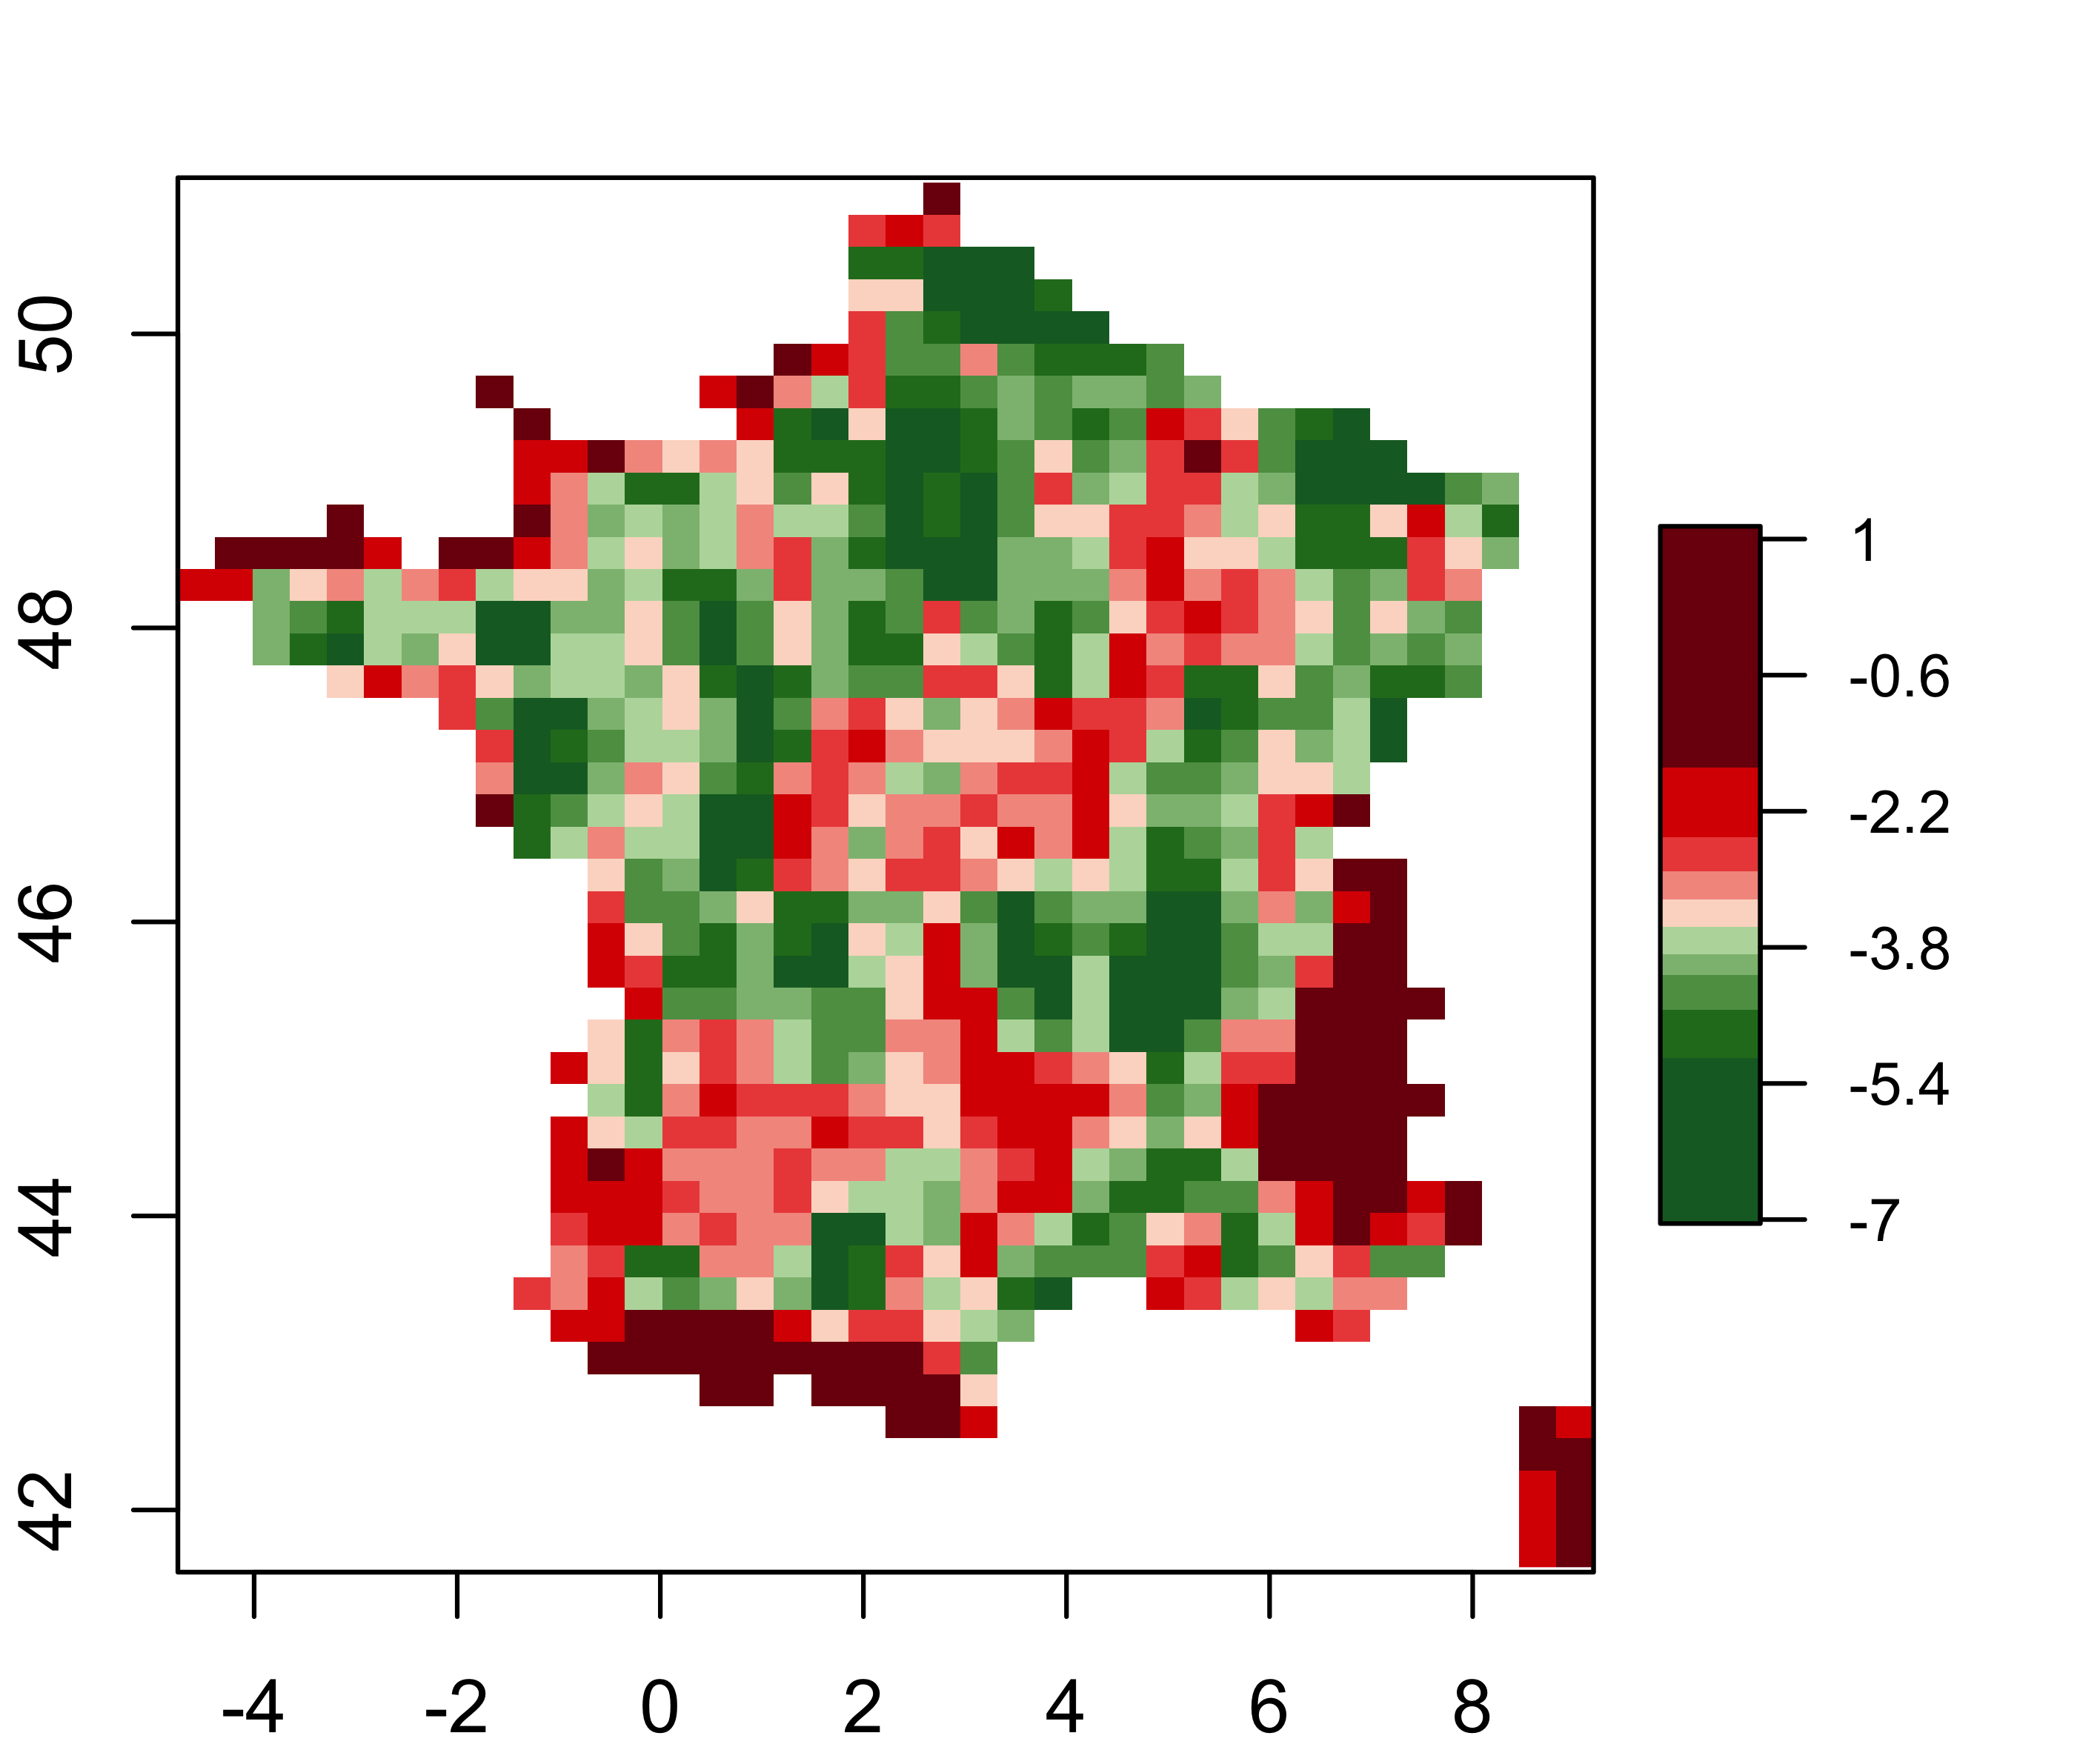
\includegraphics[width=\textwidth]{figures/morpho_corr_PCA_rhoasize12.png}

\column{0.3\textwidth}\centering
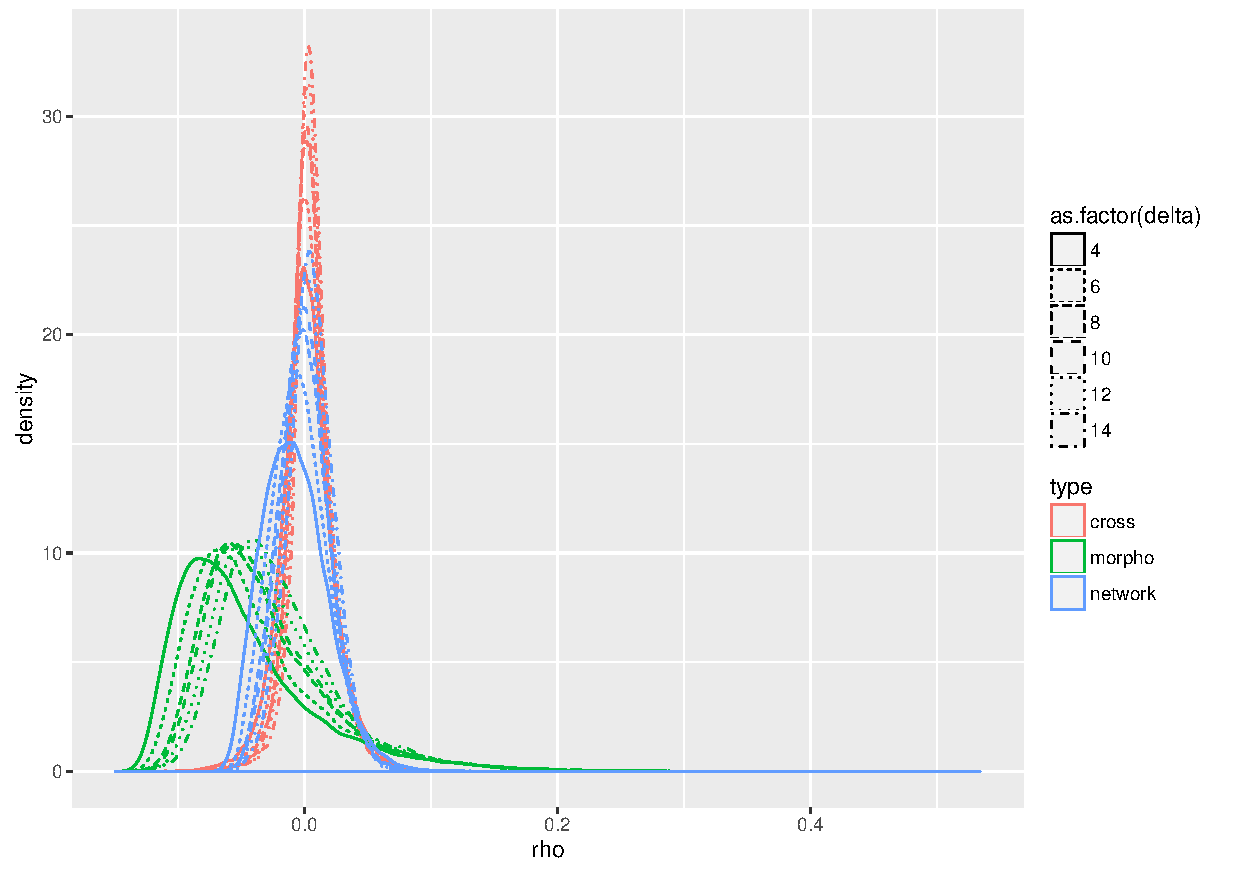
\includegraphics[width=\textwidth]{figures/morpho_corrs-distrib_varyingdelta_bytype.pdf}\\
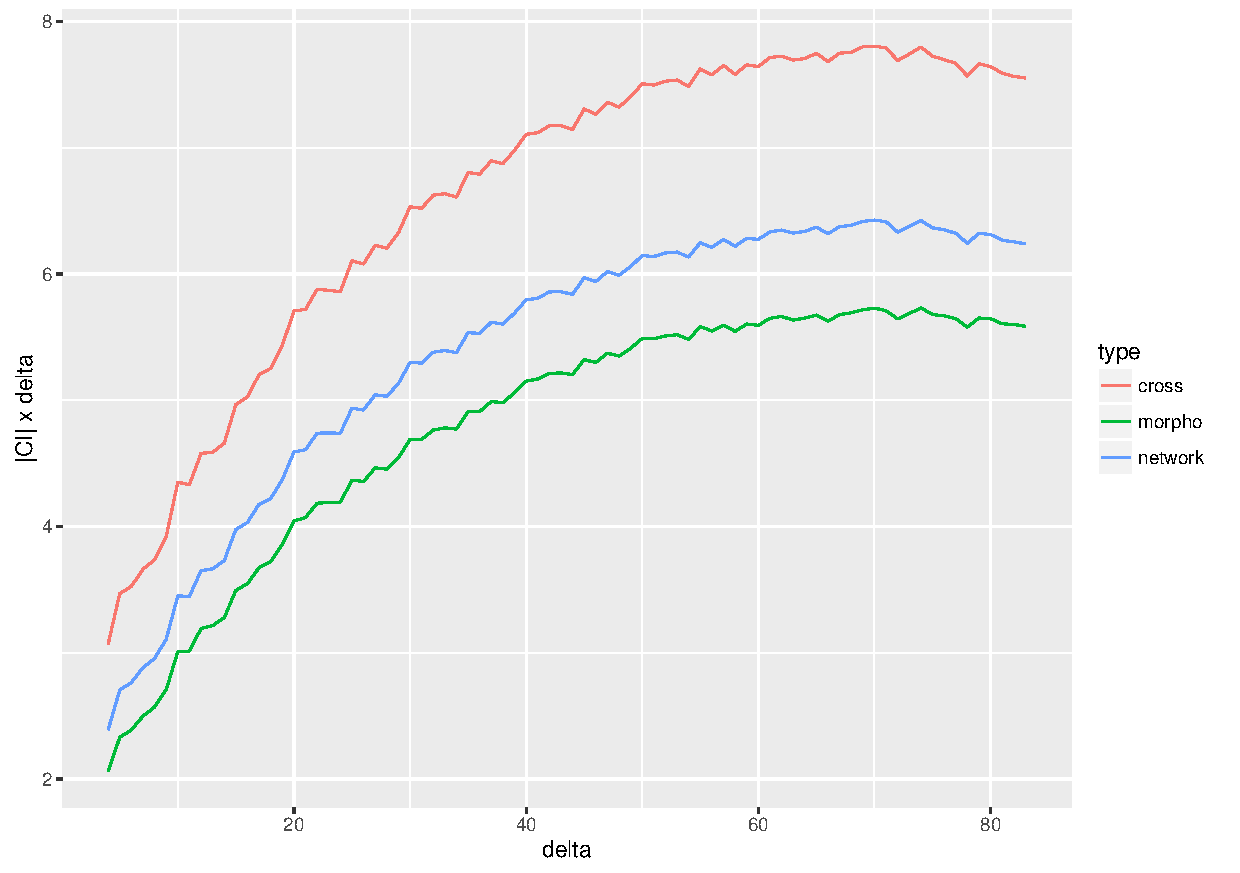
\includegraphics[width=\textwidth]{figures/corr_normalized_CI_delta}
\end{columns}

%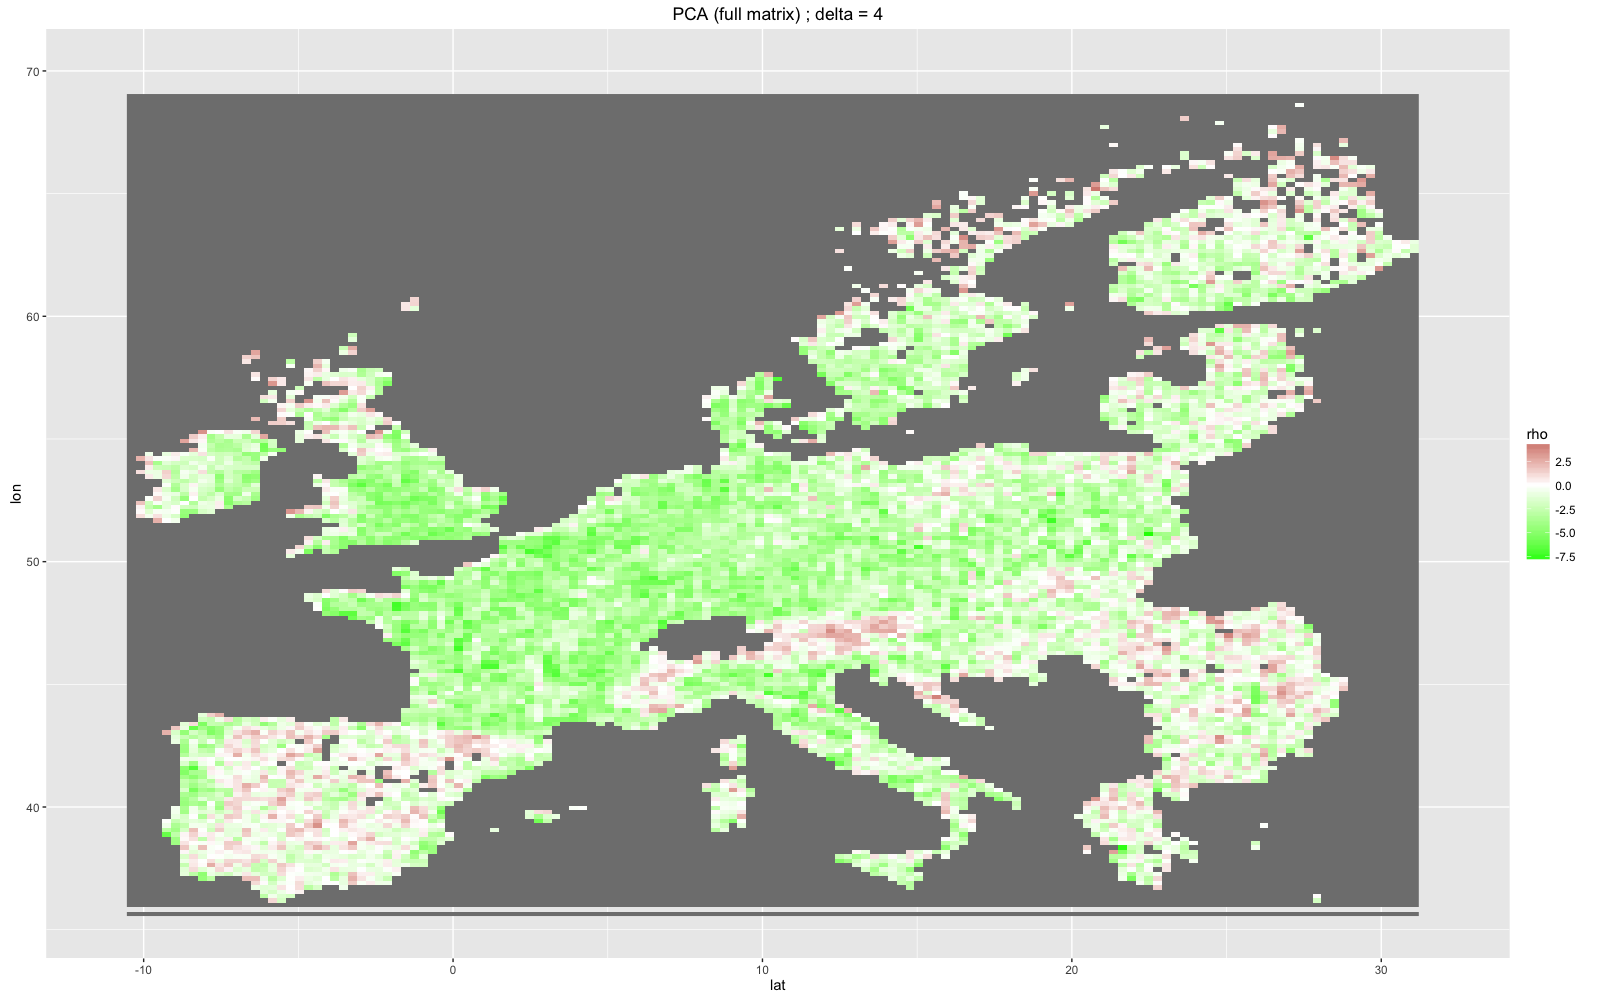
\includegraphics[width=0.5\textwidth]{figures/corr_corr_PCA_delta4}\\


\centering

%morpho_cluster_map_k5_full.png
%morpho_corr_PCA_rhoasize12.png
%morpho_indics_morpho_discrquantiles.png
%morpho_indics_network_selected_2_discrquantiles.png
%


}



%%%%%%%%%%%%
%% Modeling




%\paragraph{Modélisation}
%A l'échelle mesoscopique, des processus d'agrégation-diffusion ont été prouvés suffisant pour reproduire un grand nombre de formes urbaines avec un faible nombre de paramètres, calibrés sur l'ensemble du spectre des valeurs réelles des indicateurs de forme urbaine pour l'Europe. Ce modèle simple a pu, à l'occasion d'un exercice méthodologique explorant le possibilité de contrôle au second ordre de la structure de données synthétiques~\cite{raimbault2016generation}, être couplé faiblement à un modèle de génération de réseau, démontrant une grande latitude de configurations potentiellement générées. L'exploration de différentes heuristiques autonomes de génération de réseau a par ailleurs été entamée~\cite{raimbault2015labex}, pour comparer par exemple des modèles de croissance de réseau routier basés sur l'optimisation locale à des modèles inspirés des réseaux biologiques : chacun présente une très grande variété de topologies générées. A l'échelle macroscopique, un modèle simple de croissance urbaine calibré dynamiquement sur les villes françaises de 1830 à 2000 (base Pumain-Ined) a permis de démontrer l'existence d'un effet réseau de par l'augmentation de pouvoir explicatif du modèle lors de l'ajout d'un effet des flux transitant par un réseau physique, tout en corrigeant le gain dû à l'ajout de paramètres par la construction d'un Critère d'Information d'Akaike empirique~\cite{raimbault2016models}. Cet ensemble de modèles se positionne avec un objectif de parcimonie et dans une perspective d'application en multi-modélisation. Dans une démarche basée-agent plus descriptive et donc par un modèle plus complexe, \cite{le2015modeling} décrit un modèle de co-évolution à l'échelle métropolitaine (modèle Lutecia) qui inclut en particulier des processus de gouvernance pour le développement des infrastructures de transport. Même si ce dernier modèle est toujours en exploration, les premières études de la dynamique montre l'importance du caractère multi-niveau du développement du réseau de transport pour obtenir des motifs complexes de réseaux et de collaboration entre agents. L'ensemble de ces premiers efforts de modélisation, bien qu'ils ne soient pas majoritairement centrés sur des modèles de co-évolution à proprement parler, supportent les premiers fondements théoriques que nous proposons par la suite.




\sframe{Croissance Urbaine par Aggregation-diffusion}{

% Density model

{\small Calibration morphologique d'un modèle de croissance urbaine par aggrégation-diffusion : suggestion de processus Morphogénétiques autonomes.}

\smallskip

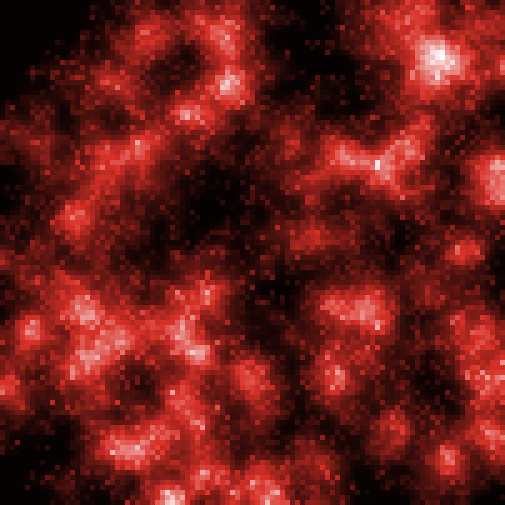
\includegraphics[width=0.24\textwidth]{figures/density_conf1}\hspace{0.1em}
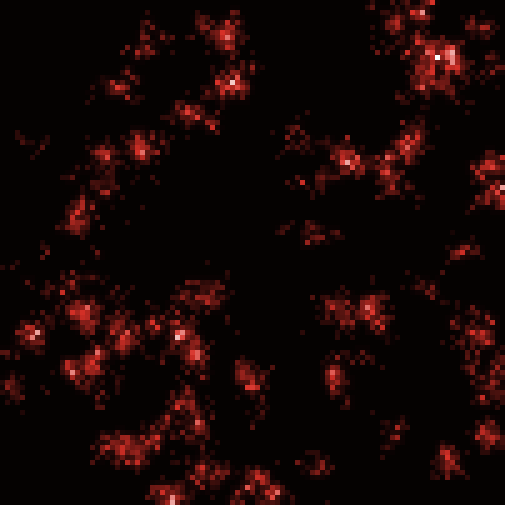
\includegraphics[width=0.24\textwidth]{figures/density_conf2}\hspace{0.1em}
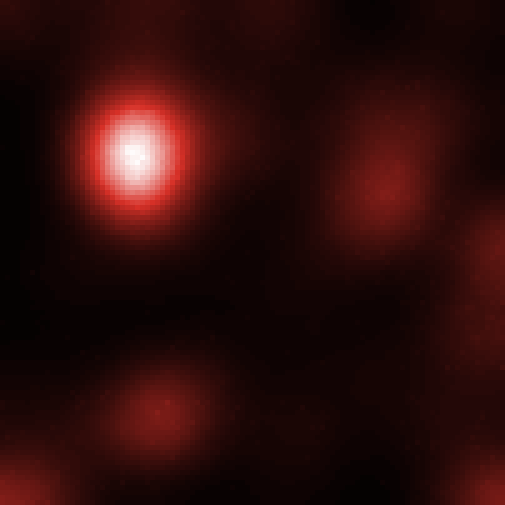
\includegraphics[width=0.24\textwidth]{figures/density_conf3}\hspace{0.1em}
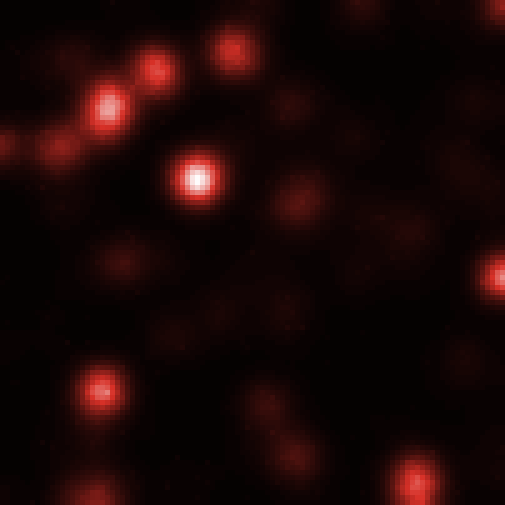
\includegraphics[width=0.24\textwidth]{figures/density_conf4}\hspace{0.1em}
\\
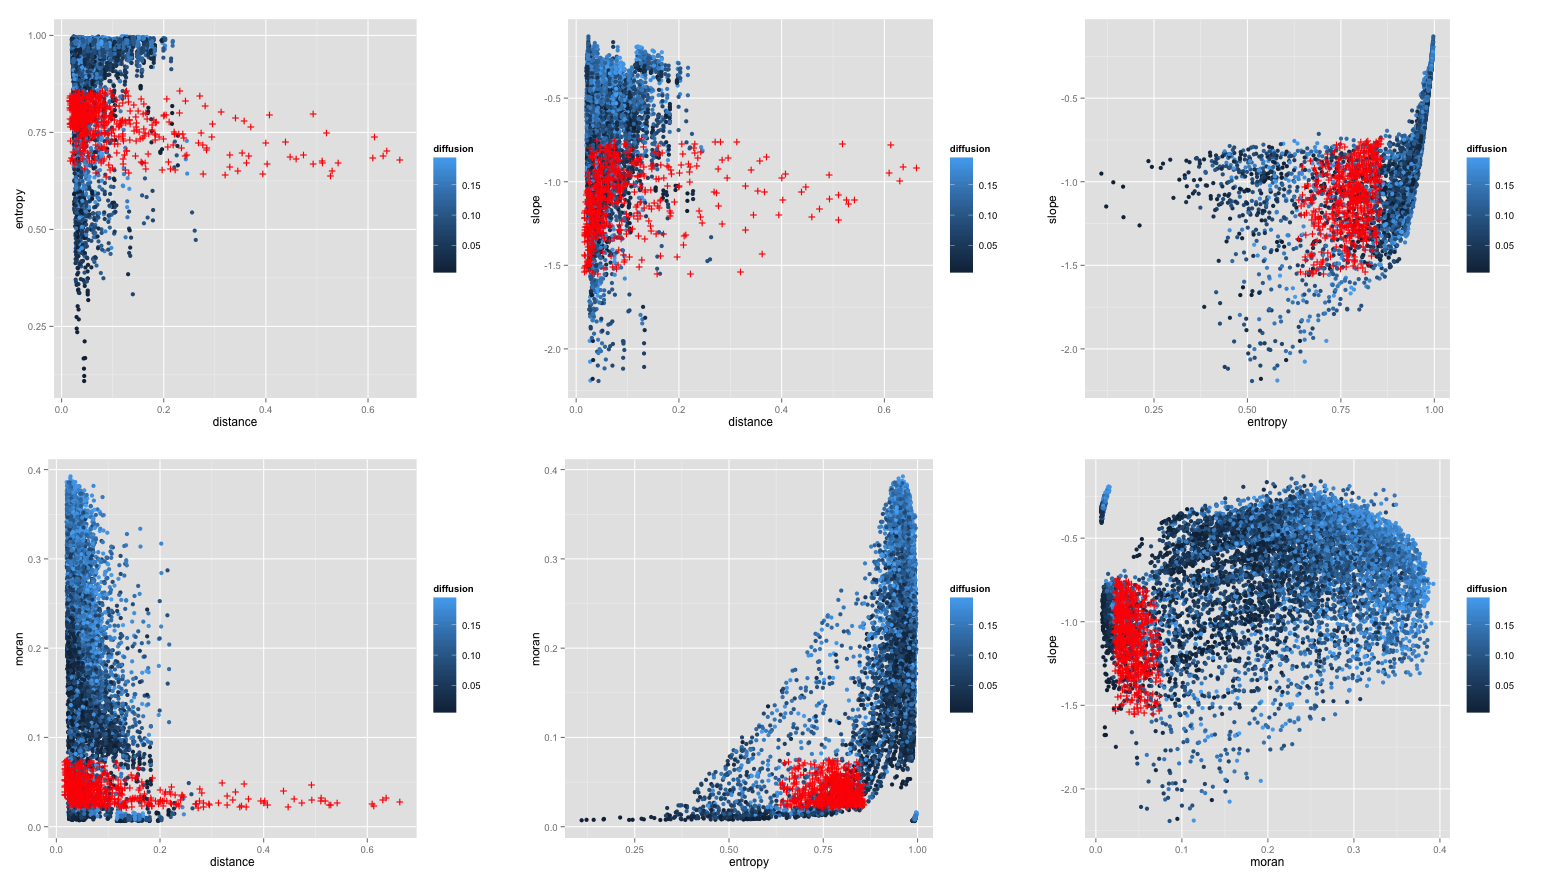
\includegraphics[width=0.5\textwidth,height=0.4\textheight]{figures/density_scatt}
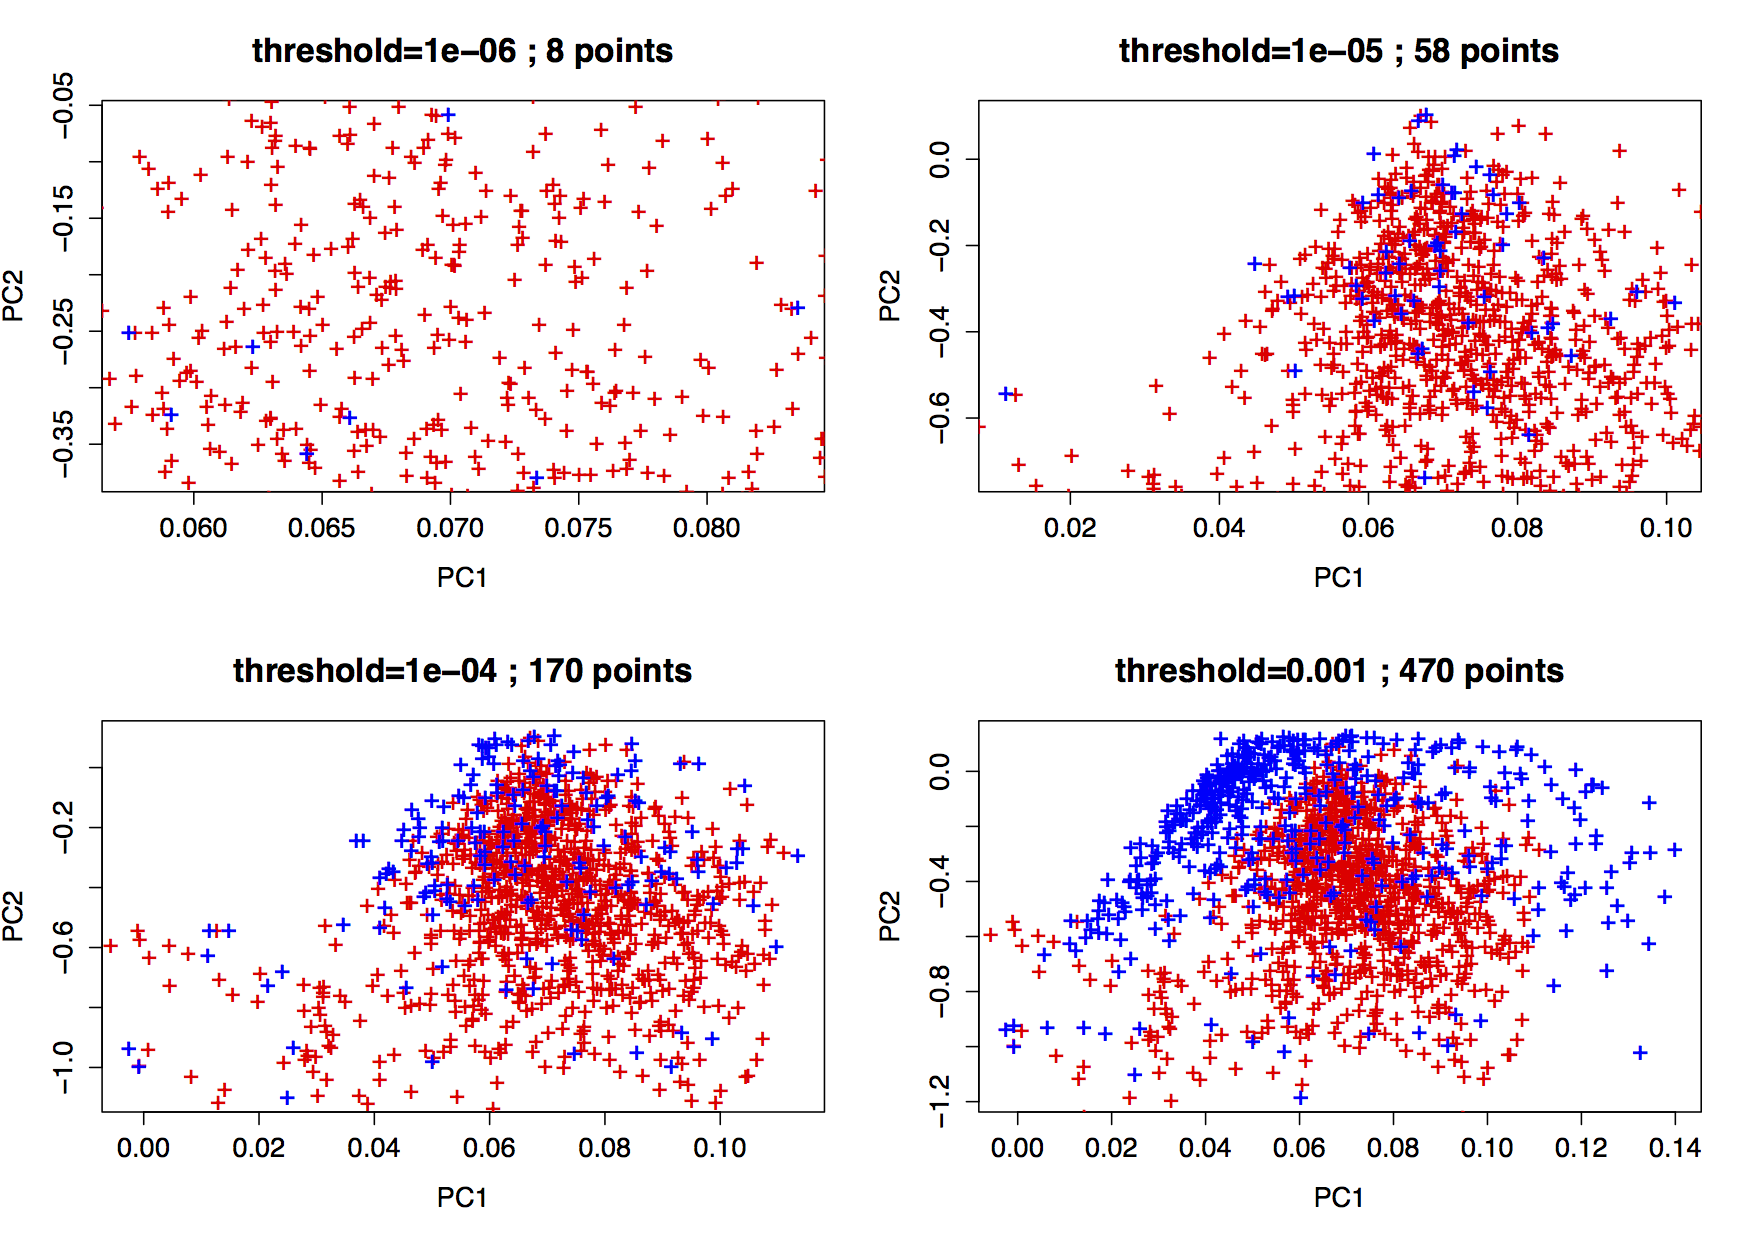
\includegraphics[width=0.5\textwidth,height=0.4\textheight]{figures/density_pca}


}




\sframe{Données synthétiques corrélées}{

Modélisation avec couplage simple montre un vaste espace faisable des correlations simulées \cite{raimbault2016generation}
 
\bigskip
 
\centering
 
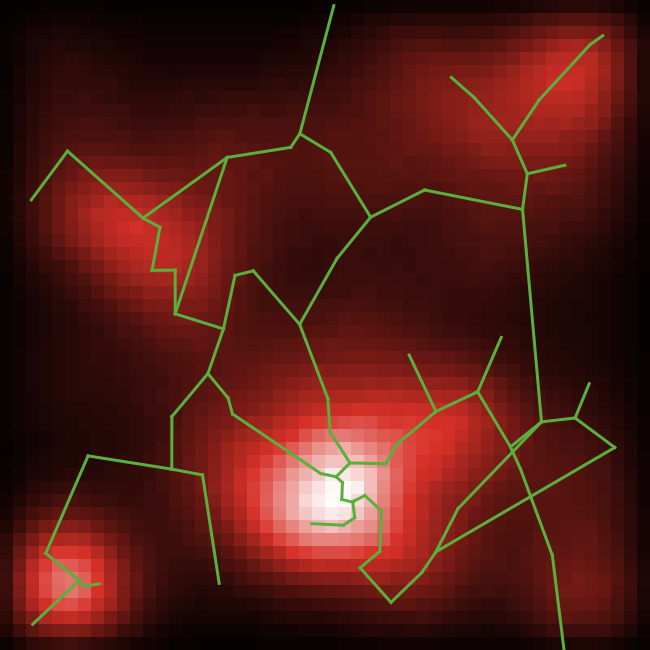
\includegraphics[width=0.48\textwidth]{figures/corr_2_param71913_seed10}\hspace{0.2cm}
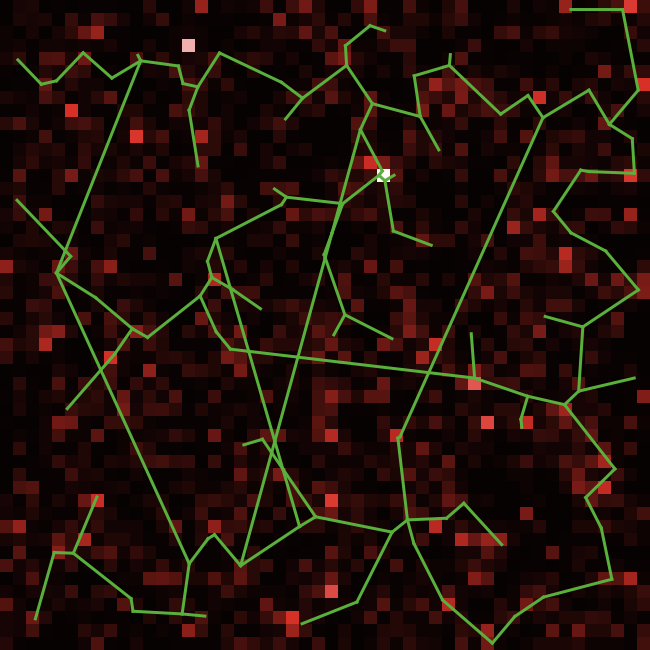
\includegraphics[width=0.48\textwidth]{figures/corr_3_param71918_seed0}

}





\sframe{Morphogenèse des Réseaux de Transport}{

Morphogenèse d'un réseau de transport et design optimal via un modèle inspiré d'un système biologique (\textit{slime mould}) \cite{raimbault2015labex}


\bigskip

\begin{columns}
\column{0.55\textwidth}
\centering
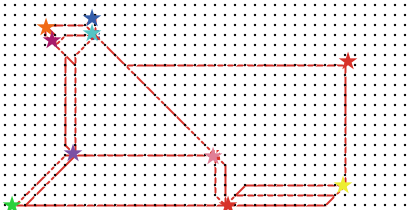
\includegraphics[width=0.9\textwidth]{figures/nwmorph_networkDense.png}

\column{0.45\textwidth}
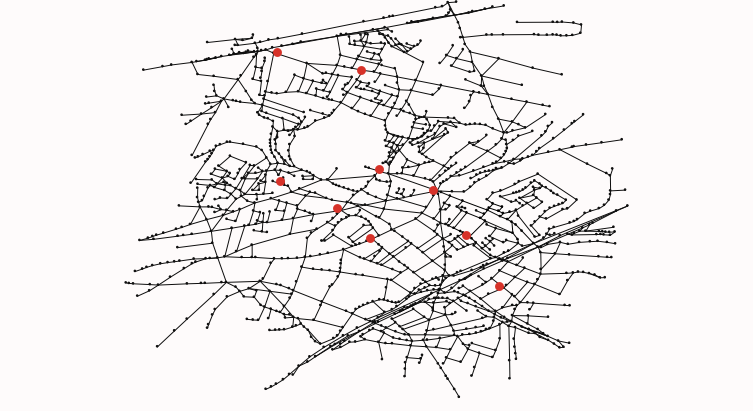
\includegraphics[width=\textwidth]{figures/nwmorph_tick1}\\
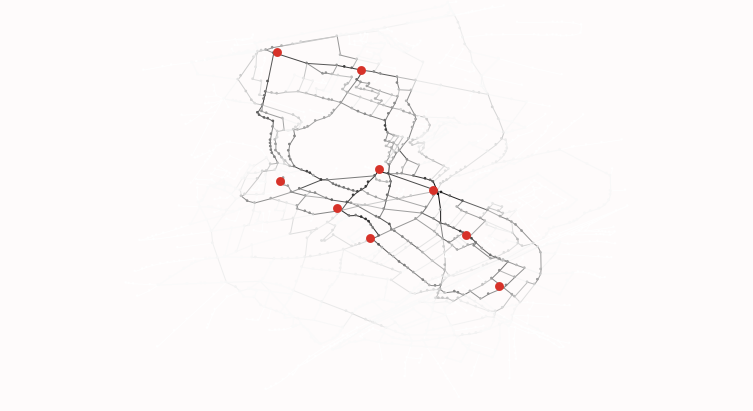
\includegraphics[width=\textwidth]{figures/nwmorph_tick101}


\end{columns}

}











\sframe{Croissance Macroscopique et Nécessité du réseau}{


\vspace{-0.4cm}

Un modèle de croissance de population à l'échelle macroscopique révèle des effets du réseau physique dans le système de villes français \cite{raimbault2016system}


\bigskip

\centering

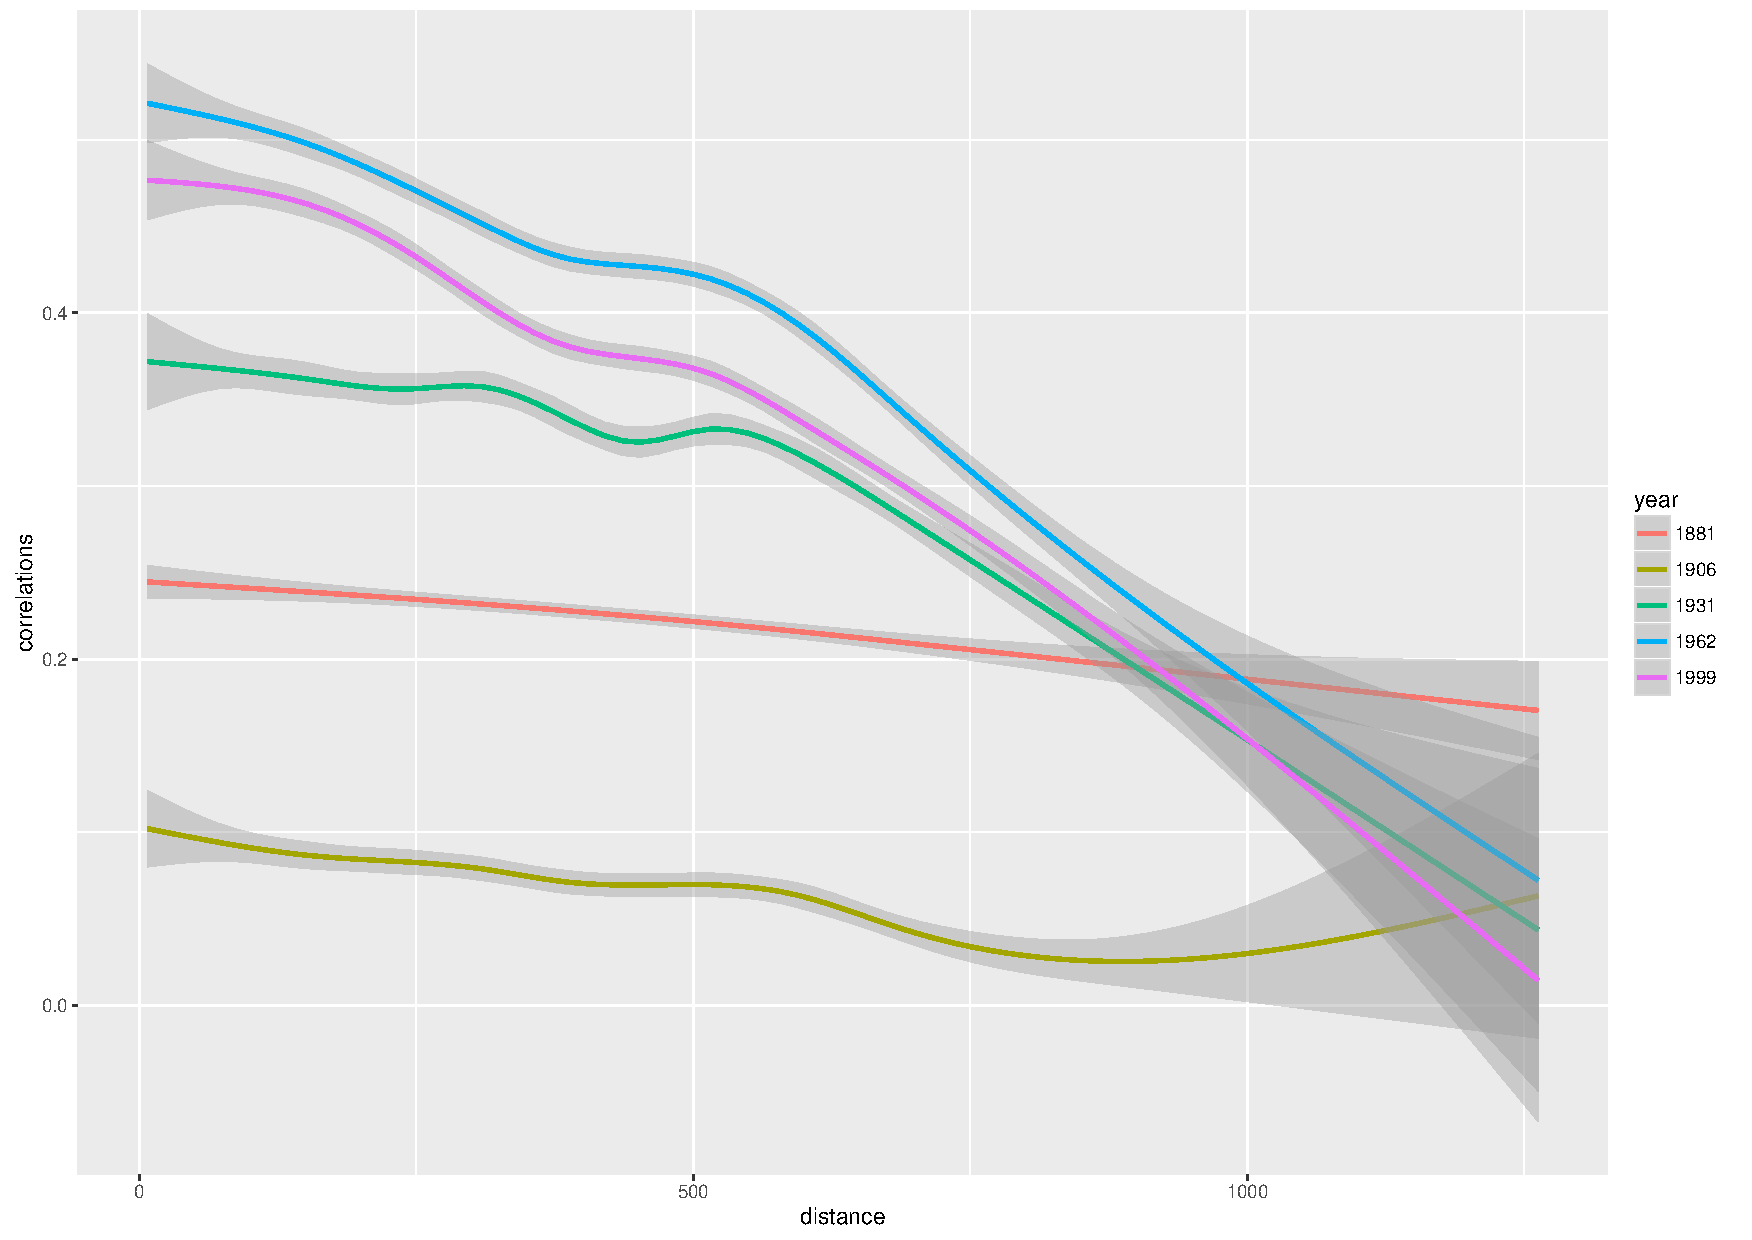
\includegraphics[width=0.35\textwidth]{figures/macro_empirical_tsCorrelations}
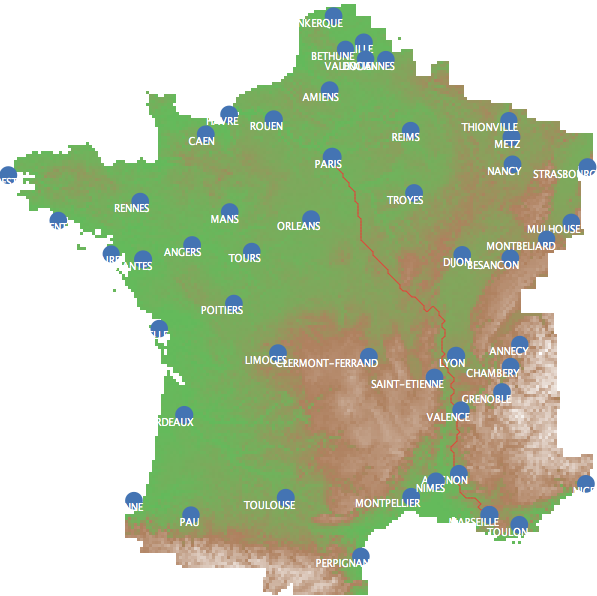
\includegraphics[width=0.25\textwidth]{figures/macro_example_shortest_path}
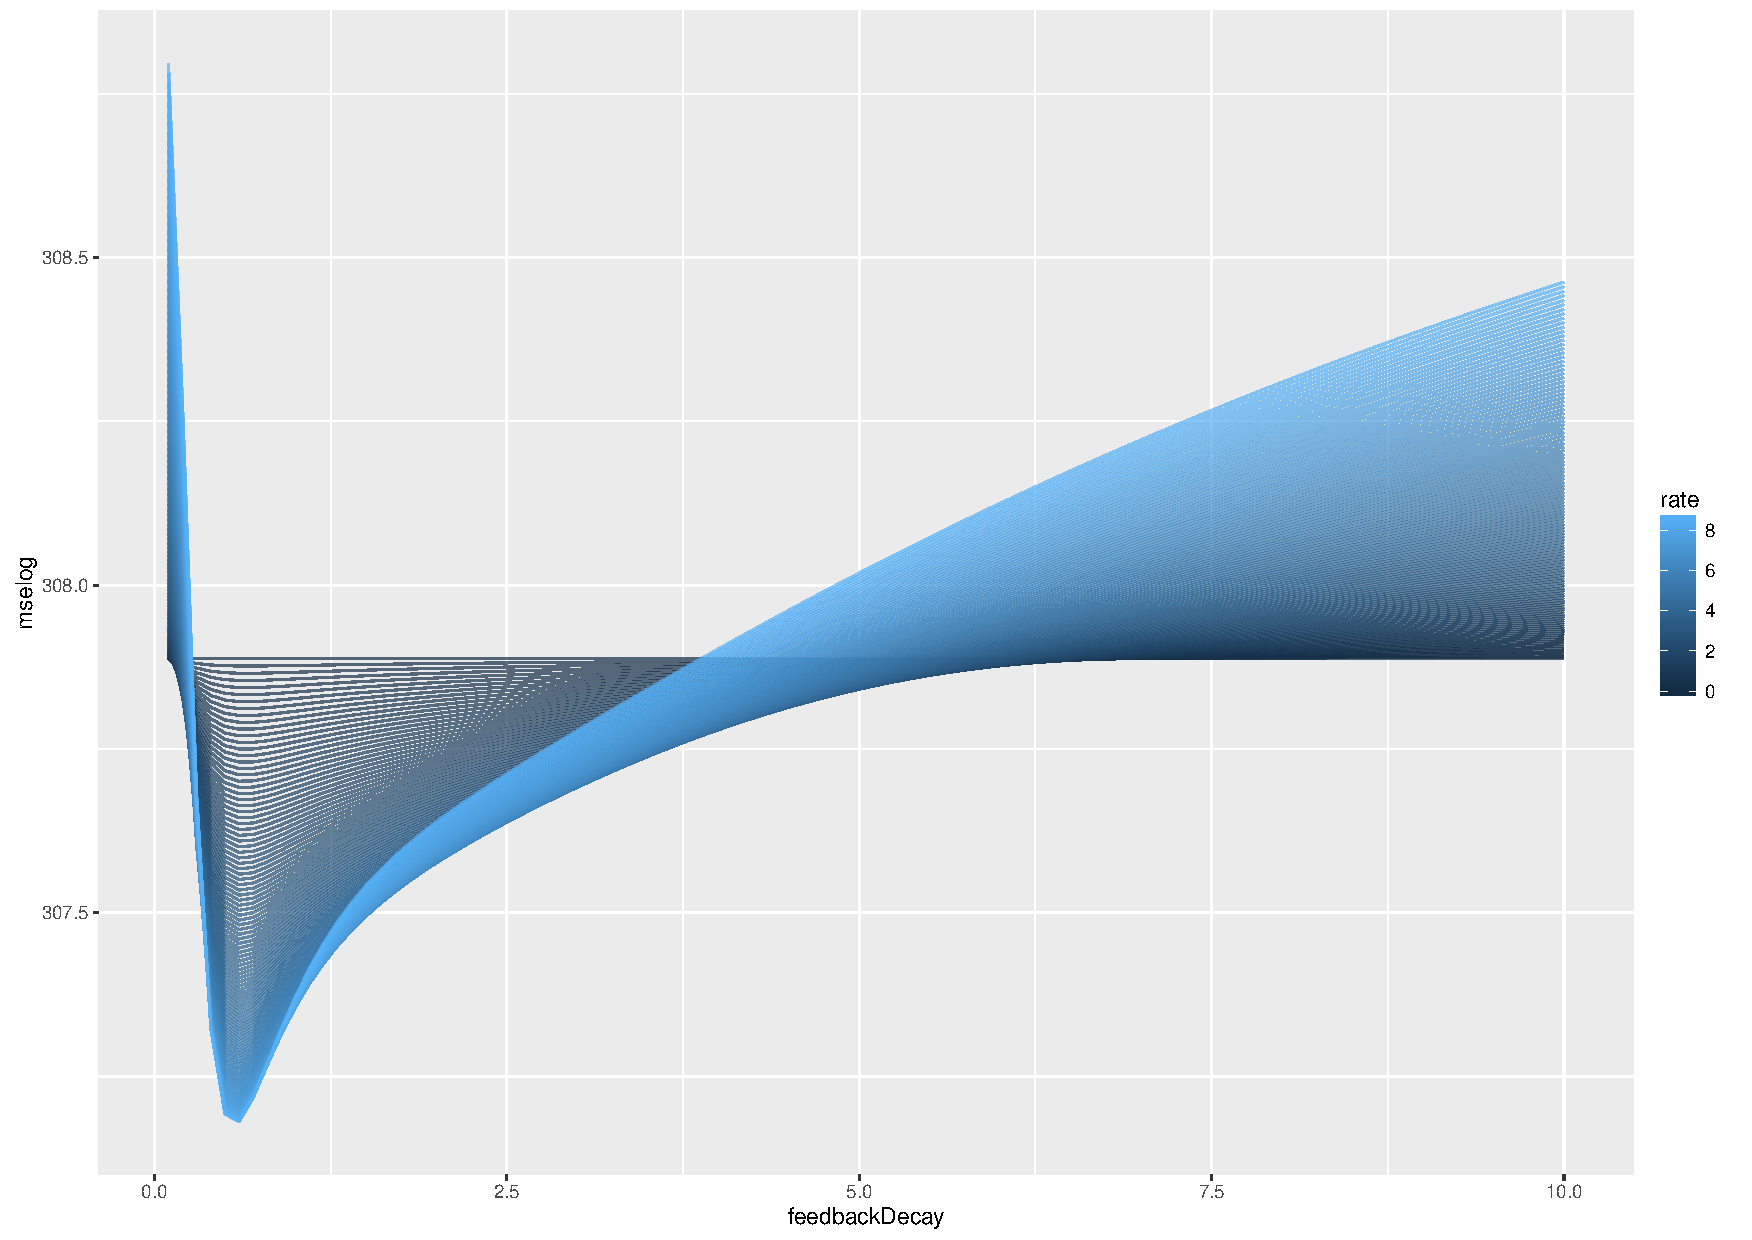
\includegraphics[width=0.35\textwidth]{figures/macro_mselog-feedbackDecay_ZOOM_fixedgravity}

}




\sframe{Croissance couplée mesoscopique}{

% RBD model : reproduces some typical urban forms

Une dynamique co-évolutionnaire simple produit des formes urbaines stylisées à une échelle mesoscopique \cite{raimbault2014hybrid}

\bigskip

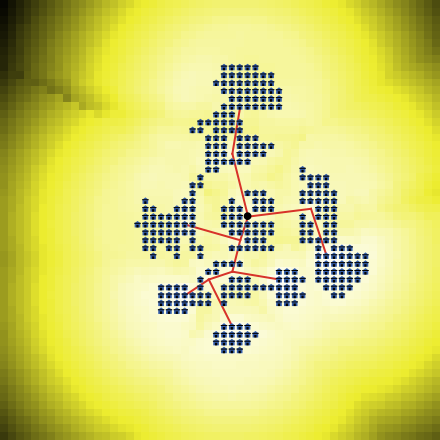
\includegraphics[width=0.3\textwidth]{figures/RBD_lattice}
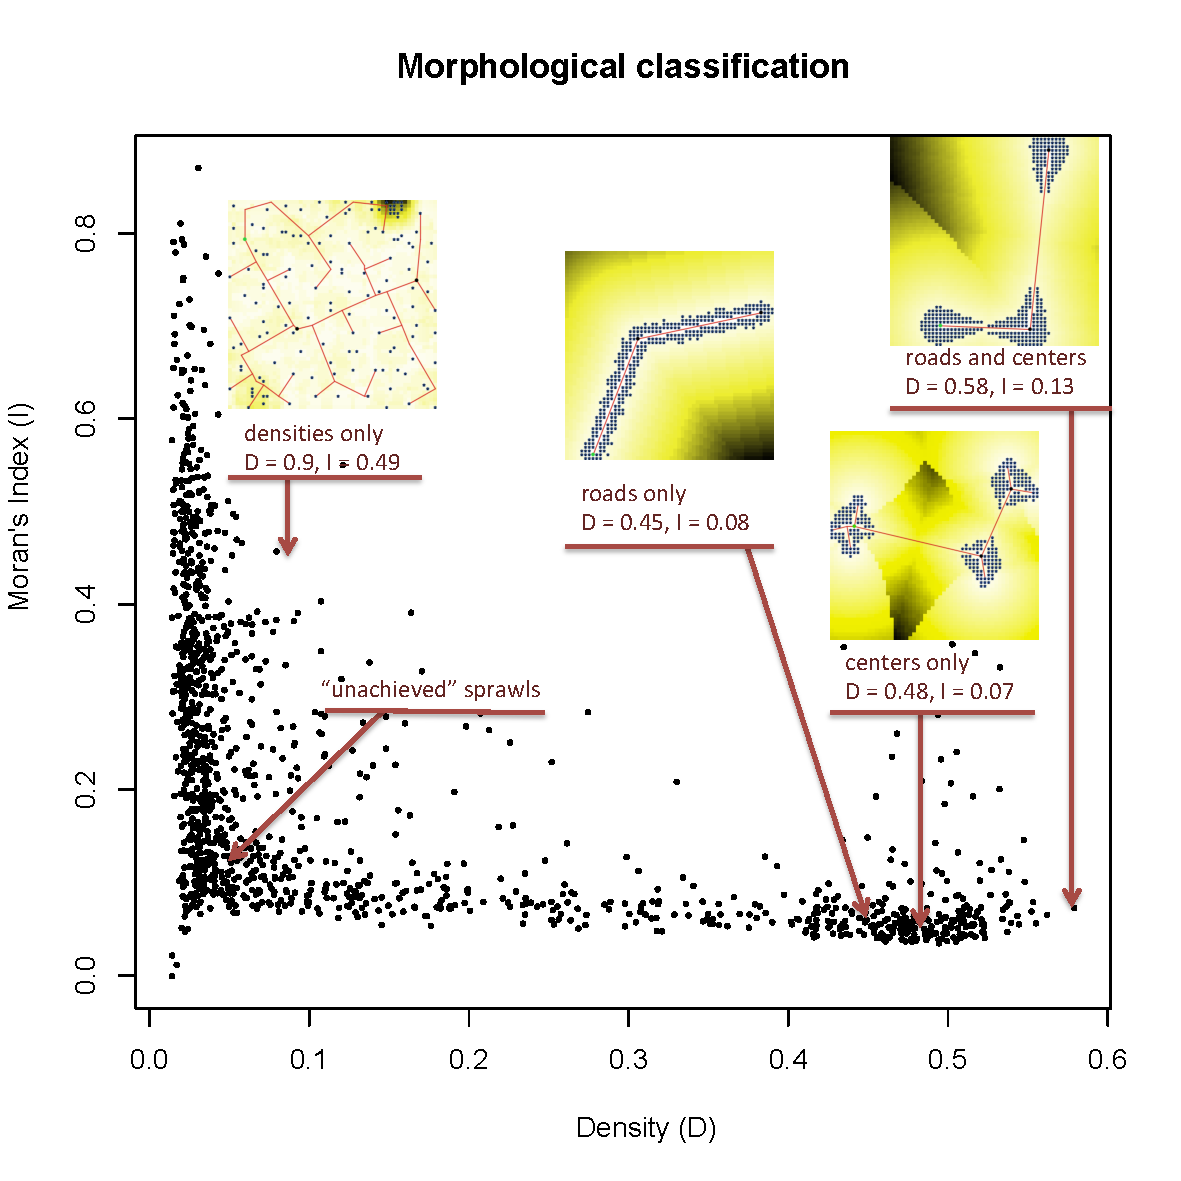
\includegraphics[width=0.35\textwidth]{figures/RBD_morpho}
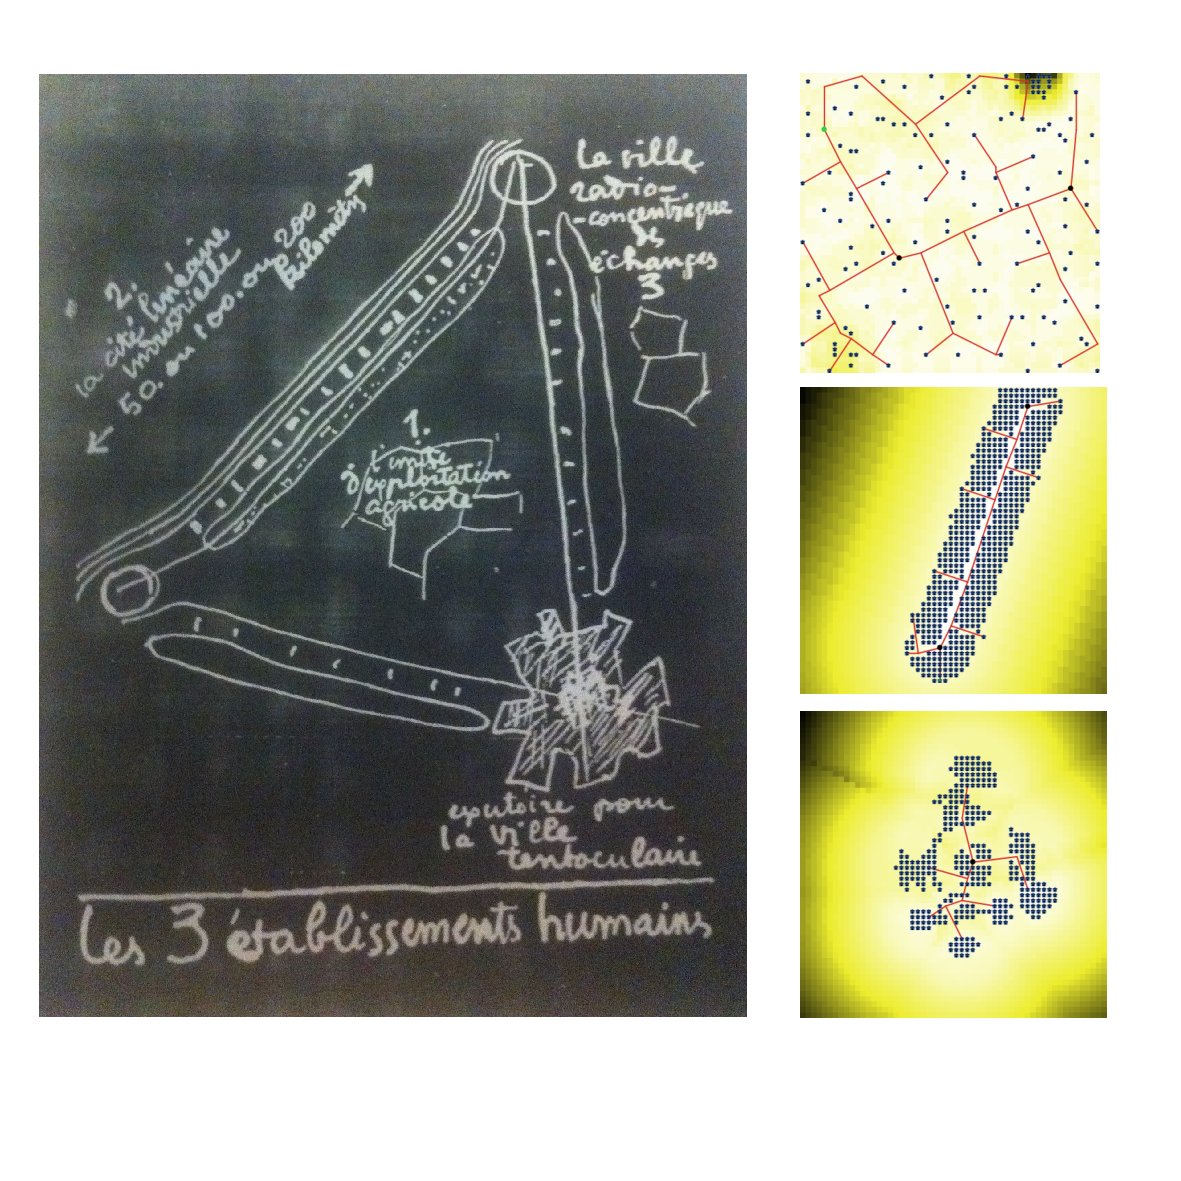
\includegraphics[width=0.35\textwidth]{figures/RBD_corbu}

\bigskip

\textit{Développements en cours : }Régimes de causalités clairement identifiables

}

%\sframe{Identification de régimes de causalités}{
% -> do not include, as under review
%}











%%%%%%%%%%%%%%%%%
\section{Construction Théorique}
%%%%%%%%%%%%%%%%%




%\paragraph{Construction d'une Théorie Géographique}
%En se basant sur les travaux précédents, nous proposons de joindre deux entrées pour la construction d'une théorie géographique ayant un focus privilégié sur les interactions entre territoires et réseaux.


%%%%%%%%%%%%%%%%%%%%%%%%%%%%
\sframe{Piliers de la Théorie}{

\justify


Vers une Théorie des Systèmes Territoriaux Co-évolutifs en Réseau\\\cite{raimbault2016towards} : fils directeurs des travaux précédents s'articulent en deux axes.

\bigskip

\begin{enumerate}
\item \textit{Morphogenèse Urbaine} $\rightarrow$ La Morphogenèse comme des règles autonomes pour expliquer la croissance de la forme urbaine : fournit des décompositions modulaires.
\item \textit{Systèmes Territoriaux co-évolutifs} $\rightarrow$ Importance du caractère non-stationnaire, hétérogène, multi-scalaire des systèmes urbains, contenu dans une approche en tant que Systèmes Complexes Adaptatifs.
\end{enumerate}

}
%%%%%%%%%%%%%%%%%%%%%%%%%%%%


%La première est par la notion de \emph{morphogénèse}, qui a été explorée d'un point de vue interdisciplinaire dans~\cite{antelope2016interdisciplinary}. Pour notre part, la morphogénèse consiste en l'émergence de la forme et de la fonction, via des processus locaux autonomes dans un système qui exhibe alors une architecture auto-organisée. La présence d'une fonction et donc d'une architecture distingue les systèmes morphogénétiques de systèmes simplement auto-organisés (voir~\cite{doursat2012morphogenetic}). De plus, les notions d'autonomie et de localité s'appliquent bien à des systèmes territoriaux, pour lesquels on essaye d'isoler les sous-systèmes et les échelles pertinentes. Les travaux sur la génération de forme urbaine calibrée par des processus autonomes, les premiers travaux sur la génération de réseaux par de multiples processus également autonomes, et des travaux plus anciens étudiant un modèle simple de morphogénèse urbaine qui suffisait à reproduire des motifs de forme stylisés~\cite{raimbault2014hybrid}, nous suggèrent la possible existence de tels processus au sein des systèmes territoriaux. 




%%%%%%%%%%%%%%%%%%%%%%%%%%%%
\sframe{Morphogenèse}{

\justify

\textit{Construction d'une définition interdisciplinaire de la Morphogenèse dans \cite{antelope2016interdisciplinary}}

\bigskip

\textbf{Morphogenèse d'un système : } Emergence de la forme et de la fonction par relations causales circulaires entre les deux, souvent autonomes entre les niveaux d'émergence (\cite{bedau2002downward}). Présence d'une fonction : architecture émergente \cite{doursat2012morphogenetic} (différent de systèmes simplement auto-organisés).

\bigskip

$\rightarrow$ \textit{Identification de sous-systèmes et échelles pertinents dans les systèmes territoriaux}


}
%%%%%%%%%%%%%%%%%%%%%%%%%%%%


% Théorie évolutive des villes
%D'autre part, le cadre d'un théorie évolutive des villes est plébiscité par nos résultats empiriques, qui montrent le caractère non-stationnaire, hétérogène, multi-scalaire des systèmes urbains. Pour rester le plus général possible, et comme nos résultats à la fois empiriques et de modélisation (génération de formes quelconques par le modèle d'agrégation-diffusion par exemple) s'appliquent aux systèmes territoriaux en général, nous nous plaçons dans le cadres de territoires humains de Raffestin~\cite{raffestin1988reperes}, c'est à dire ``la conjonction d'un processus territorial avec un processus informationnel'', qui peut être interprété dans notre cas comme le système complexe socio-techno-environmental que constitue un territoire et les agents et artefacts qui y interagissent. L'importance des réseaux est soulignée par nos résultats sur la nécessité du réseau dans le modèle de croissance macroscopique : nous proposons alors de parler de \emph{Systèmes Territoriaux Complexes en Réseaux}, en ajoutant au plongement du territoire dans la théorie évolutive la particularité qu'il existe des composantes cruciales qui sont les réseaux (de transport en l'occurrence), dont l'origine peut être expliquée par la théorie territoriale des réseaux de Dupuy~\cite{dupuy1987vers}.


%%%%%%%%%%%%%%%%%%%%%%%%%%%%
\sframe{Systèmes Territoriaux Complexes en Réseaux}{

\textit{Définition des systèmes territoriaux}

\bigskip

\begin{itemize}
\item \textit{Théorie Evolutive Urbaine} $\rightarrow$ Systèmes de Villes comme Systèmes Complexes Adaptatifs, appliquée aux établissements humains en général et ainsi aux systèmes territoriaux.
\item \textit{Territoires Humains en Réseau} $\rightarrow$ Approche Raffestinenne du territoire~\cite{raffestin1988reperes} (``\textit{conjonction d'un processus territorial avec un processus informationnel}''), combinée à la théorie des réseaux de Dupuy~\cite{dupuy1987vers} (réalisation de réseaux transactionnels).
\item \textit{Co-évolution} $\rightarrow$ Co-évolution comme l'existence de \textit{niches}, conséquence de motifs de frontières et signaux~\cite{holland2012signals}.
\end{itemize}

\bigskip


%\textbf{Definition : } Territorial systems are networked Human Territories. They are multi-level complex adaptive systems following Evolutive Urban Theory.


}


%Nous spéculons alors l'hypothèse suivante afin de réconcilier nos deux approches : \textbf{l'existence de processus morphogénétiques dans lesquels les réseaux ont un rôle crucial est équivalente à la présence de sous-systèmes dans les systèmes territoriaux complexes en réseaux, qu'on définit alors comme co-évolutifs.} Cette proposition a de multiples implications, mais devrait guider notamment les travaux de modélisation vers une méthodologie modulaire et de multi-modélisation afin d'essayer d'exhiber des processus morphogénétiques, et les travaux empiriques vers une étude plus poussée des correlations, causalités (dans le cas de séries temporelles) et recherche de décompositions modulaires des systèmes.





%%%%%%%%%%%%%%%%%%%%%%%%%%%%
\sframe{Formulation de la Théorie}{



\textbf{Hypothèse : } \textit{l'existence de processus morphogénétiques dans lesquels les réseaux ont un rôle crucial est équivalente à la présence de sous-systèmes dans les systèmes territoriaux complexes en réseaux, qu'on définit alors comme co-évolutifs.}

% implications


\bigskip

\textbf{Implications}

\medskip

$\rightarrow$ Modélisation vers une méthodologie modulaire et de multi-modélisation afin d'exhiber des processus morphogénétiques

\medskip

$\rightarrow$ Travaux empiriques vers une étude plus poussée des correlations, causalités (pour les séries temporelles) et recherche de décompositions modulaires des systèmes.



}
%%%%%%%%%%%%%%%%%%%%%%%%%%%%



%%%%%%%%%%%%%%%%%%%%%%%%%%%%
\sframe{Co-évolution at the mesoscopic scale}{

% retour de la théorie vers les modèles : travaux en cours

\justify

\vspace{-0.4cm}

\textit{Retour de la théorie vers les modèles et les études empiriques}

\medskip

Multi-modélisation de la co-évolution à l'échelle mesoscopique (présentation à venir @CCS17)

\medskip

\centering

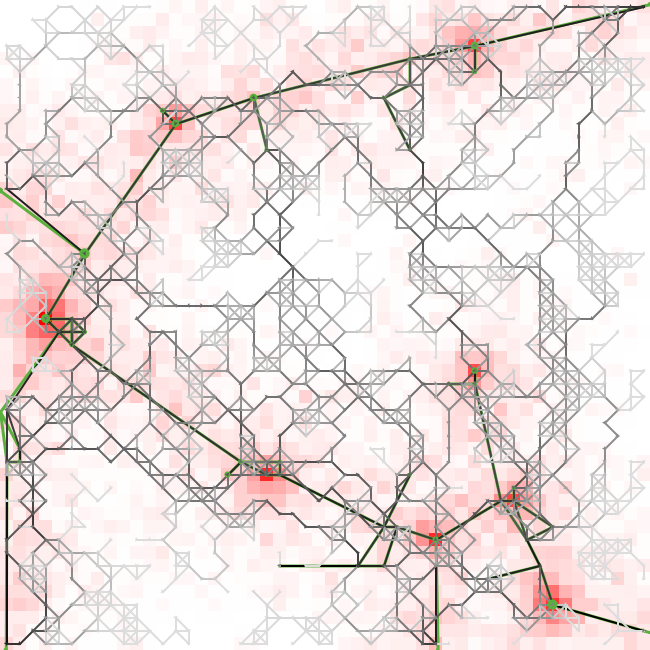
\includegraphics[width=0.45\textwidth]{figures/corr_example-bio-process-0}\hspace{0.1cm}
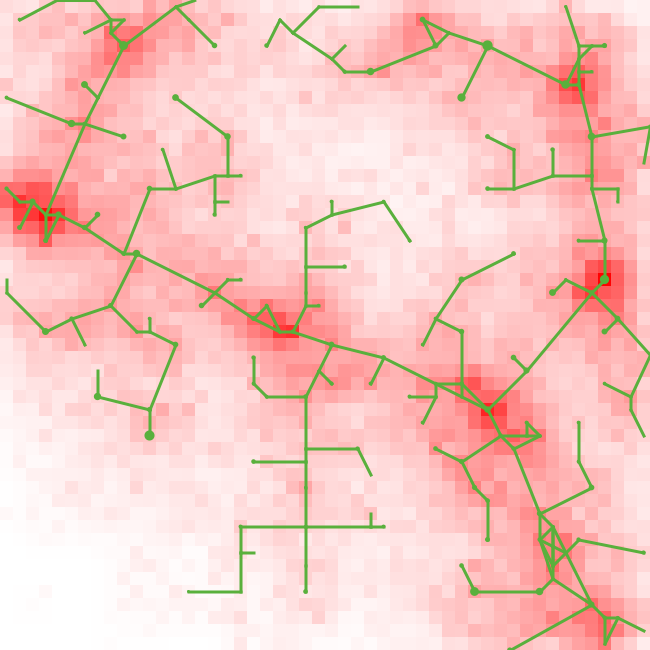
\includegraphics[width=0.45\textwidth]{figures/corr_example-heuristic-0}

}



\sframe{Lutecia}{

\vspace{-0.4cm}

Lutecia (\cite{le2015modeling}) : un modèle de co-évolution incluant les processus de gouvernance d'extension des réseaux de transport ; application à la Mega-region Urbaine du Delta de la Rivière des Perles

\medskip
\centering

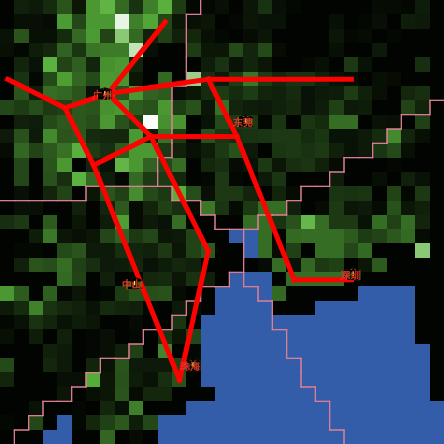
\includegraphics[width=0.4\textwidth]{figures/lutecia_exrun_2_tick0.png}\hspace{0.1cm}
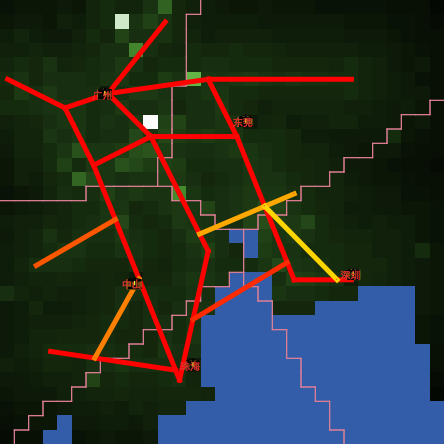
\includegraphics[width=0.4\textwidth]{figures/lutecia_exrun_2_tick6.png}

}









%\paragraph{Futurs Développements}
%Cet exercice permet d'illustrer la co-construction d'un matériel quantitatif (études empiriques et modélisation) et d'un matériel théorique, puisqu'il est clair que les directions de recherche dans chacun des points ci-dessus ont été construites progressivement, par itérations et allers-retours entre les trois domaines : la conception de modèles de simulation complexes résulte d'un cadre théorique englobant les paradigmes de la complexité, la recherche empirique de propriétés de non-stationnarité également, tandis que les modèles hybrides sont construits et calibrés par les faits stylisés et données empiriques. Notre théorie est bien sûr bien loin d'être mature, mais son existence permet déjà de guider les analyses quantitatives suivantes (modèles fortement couplés ; tests de causalités dans les données spatio-temporelles; etc.) qui seront alors crucial pour la co-évolution de l'ensemble par la suite. L'essence de la Géographie Théorique et Quantitative réside dans cette co-production qui transcende les oppositions classiques entre quantitatif et qualitatif, et à laquelle nous prétendons que participent également les outils et les méthodes : toute perspective scientifique est une combinaison de chacune des dimensions, qui à chaque fois jouent un rôle différent dans la co-évolution. L'illustration de cette proposition de manière plus précise fera également l'objet de travaux futurs.






\sframe{Discussion}{

% discussion
%  Idées
%
% - importance de la reflexivité ? meta-théories, production de connaissance, etc ?
% - développements under review : évoquer le grd Paris et les régimes de causalité ; analyse de la th. evolutive ? ; gaz price.

\justify

$\rightarrow$ Développements empiriques en cours, guidés par la construction théorique : régimes de causalités dans le modèle RBD ; causalités territoriales autour du Grand Paris Express ; Analyse spatio-temporelle des prix de vente de l'essence.


\medskip

$\rightarrow$ Importance du positionnement dans le cadre de connaissance : allégorie de la TQG qui permet de mieux la comprendre ?

\medskip

$\rightarrow$ Rôle de la Réflexivité : la méta-théorie présente des similitudes structurelles avec la théorie (co-évolution et morphogenèse). Besoin de théories reflexives/récursives pour les Systèmes Complexes ?

}




\sframe{Conclusion}{

\justify

$\rightarrow$ Une illustration de la construction itérative et des allers-retours entre les différents domaines de connaissance en TQG (ou plutôt en \emph{Géographie Intégrée} car lecture par notre prisme épistémologique propre).

\bigskip

$\rightarrow$ Permet de tendre vers une plus grande intégration horizontale (questions transversales), verticale (disciplines intégrées) - cf. Roadmap Systèmes Complexes~\cite{2009arXiv0907.2221B} - et des domaines de connaissance.

\bigskip
\bigskip
\bigskip


\footnotesize{ - Code et données des différentes études mentionnées disponible sur github à\\ \texttt{https://github.com/JusteRaimbault}
}

}






\sframe{Reserve slides}{

\centering

\Large

\textbf{Reserve Slides}

}




\sframe{Fondements Epistémologiques du Cadre de Connaissances}{

% Perspectivisme de Giere
%   Giere : explaining Science
%   Feyereabend justifying perspectivism ?
% positionnement % Hacking ?

%  // link with formal framework socio-eco systems ? -> in dvlpmt ?

% Pour une épistémologie appliquée ?

\justify

1. Une approche cognitive de la Science~\cite{giere2010explaining} : les \textit{agents} scientifiques~\cite{giere2010agent} à l'origine des dynamiques co-évolutives des connaissances. Cadre épistémologique du perspectivisme~\cite{giere2010scientific}.

\bigskip

2. Compatible avec une \textit{science anarchiste} à la Feyerabend \cite{feyerabend1993against} : auto-organisation et émergence des connaissances


\bigskip

3. Extrême sur la ``check-list'' de Hacking~\cite{hacking1999social} (au delà de Kuhn) :
\footnotesize
\begin{itemize}
\item contingence maximale de par la nature dépendante au chemin du processus complexe de co-évolution des connaissances
\item degré de constructivisme maximal dans la posture perspectiviste
\item stabilité des sciences fortement couplée entre origine interne et externe de par le rôle des agents
\end{itemize}


}




\sframe{Formulation (I)}{

% specification and definitions

% first def co-evol and morphogenesis

\justify

\vspace{-0.5cm}

\textbf{Definition.} La morphogenèse d'un système implique des relations circulaires causales et souvent autonomes entre les niveaux d'émergence\\ (\cite{bedau2002downward}) entre \textit{forme} et \textit{fonction} \cite{antelope2016interdisciplinary}, et exhibe dans ce sens une architecture émergente \cite{doursat2012morphogenetic}.

\bigskip

\textbf{Fait stylisé.} Il existe des processus de production de connaissances scientifiques morphogénétiques, constitués d'ensemble de \textit{perspectives}, et impliquant une co-évolution des vecteurs (agents) et de domaines de connaissance (def. ci-dessous).

\bigskip

\textbf{Postulat.} La TQG en fait majoritairement partie et est en ce sens précurseur d'une \textit{Géographie Intégrée}. [Note : appel aux épistémologues, démonstration systématique à effectuer]





}


\sframe{Formulation (II)}{

\textbf{Définition des domaines.}

\begin{itemize}
\item \textbf{Empirique} Connaissances empiriques sur des cas réels
\item \textbf{Théorique} Construction cognitives plus générales
\item \textbf{Modélisation} \textit{Medium} formalisé de la perspective, ou tout modèle au sens de Varenne \cite{varenne2010simulations}
\item \textbf{Données} Information brute qui a été captée
\item \textbf{Méthodes} Structures génériques de production de connaissances
\item \textbf{Outils} Proto-méthodes et supports des autres domaines
\end{itemize}


\medskip

\textbf{Corolaire.} La distinction entre ``quantitatif'' et ``qualitatif'' est arbitraire et sans intérêt pour la production dans ce cadre, de par la nécessité de l'ensemble de leur composantes dans l'ensemble des domaines.  


}



\sframe{Illustration}{

%\footnotesize\textit{Projection of knowledge space as a complete graph (tentative qualifications for binary relations)}

\footnotesize\textit{Projection de l'espace des connaissances comme graphe complet (qualifications arbitraires pour les relations binaires)}


%\medskip

\centering

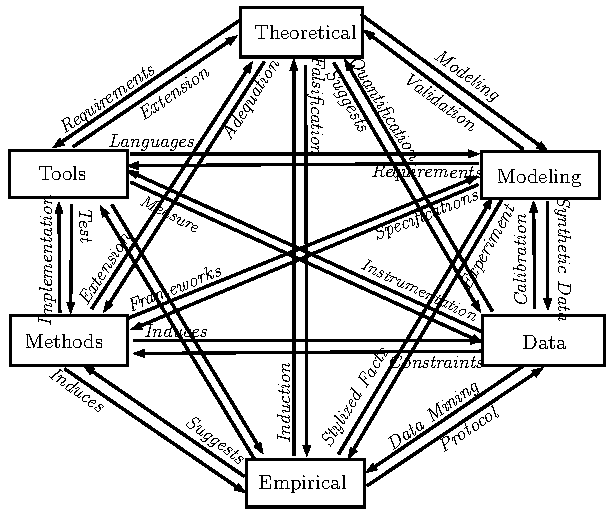
\includegraphics[width=0.7\textwidth]{figures/tqg}

}





\sframe{Implémentation du Cadre de Connaissances}{

\justify

% meta-modeling, impossibilité d'un cadre unifié, on ne cherche pas à faire du meta-modeling ni à expliquer la production de connaissance en général, mais prendre conscience du processus de co-evolution et de tirer parti de cette prise de conscience.

% sur le meta-modeling, note sur reflexivité-strange loops ?

% \cite{Fanelli04042017} : science ouverte
% ex. ReScience
%  quani-quali : opposer "evidence-based et quali argumenté et contextualisé" (politique InSHS) : pas pertinent.


\vspace{-0.2cm}

\textbf{Implémentation : }Cadre meta, pouvant a priori être traduit dans la plupart des conceptions du modèle

\begin{itemize}
\item Modèles de simulation
\item Modèles statistiques ou mathématiques
\item Modèles de données
\item Modèles conceptuels
\end{itemize}

\bigskip


\textbf{Science Ouverte : } Reproductibilité et transparence \textbf{totales} (sous conditions éthiques) postulées comme nécessaires (positionnement ``politique'' à ce stade, pourrait être étudié systématiquement \cite{Fanelli04042017}). Outils libres et ouverts, collaboratifs etc. (git : cf. \cite{rescience} Journal of Replicated Science)


}




\sframe{The LUTECIA Model : Rationale}{

\justify

\textit{Mega-city Regions~\cite{hall2006polycentric} exhibit new qualitative regimes of urban systems ?}

\bigskip

$\rightarrow$ A LUTI + infrastructure provision model (LUTECIA)

\medskip

$\rightarrow$ Coevolution transport / urbanism (LUTI model with endogeneous transport infrastructure provision)

\medskip

$\rightarrow$ Game theory framework to predict emergence of centralized decision within a polycentric region

\medskip

$\rightarrow$ Importance of accessibility at MCR scale

}



\sframe{The LUTECIA Model : Structure}{

LU : Land Use module ; T : Transport module ; EC : Evaluation of Centralized decision module ; I : Infrastructure provision module ; A : Agglomeration economies module

\medskip

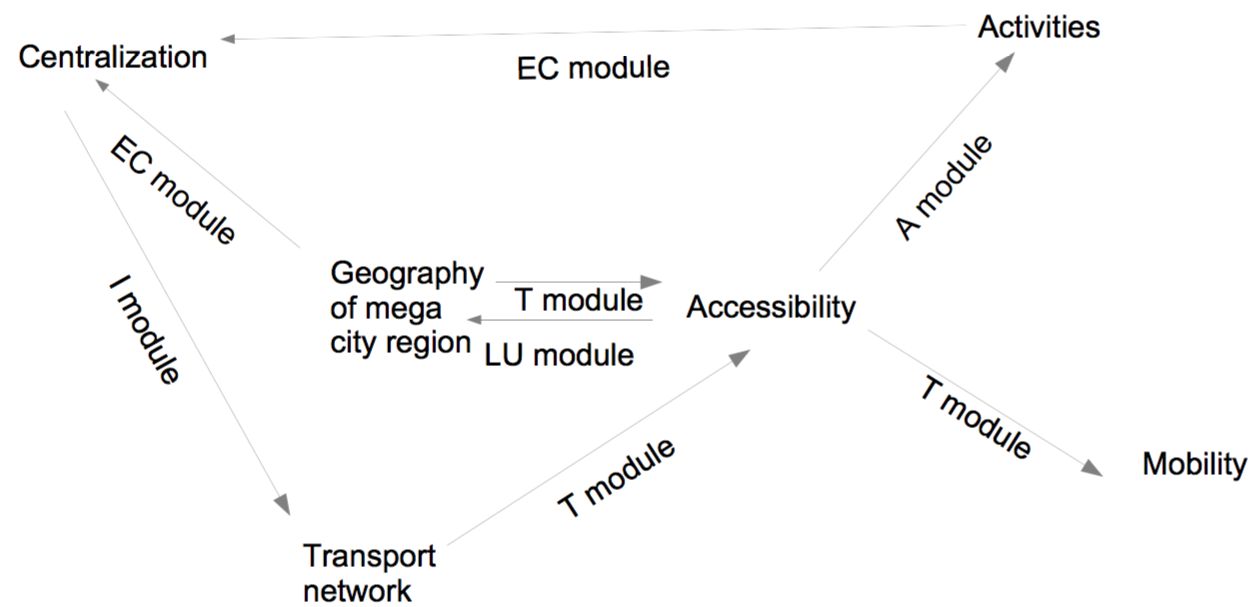
\includegraphics[width=\textwidth]{figures/lutetia_structure}

}


\sframe{Governance Modeling}{

Matrix of actors utilities, depending on respective choices

\bigskip

\begin{tabular}{ |c|c|c| } 

 \hline
 1 $|$ 2  & C & A \\ \hline
 C & $U_i = \kappa \cdot \Delta X_i(Z^{\ast}_C) - I - \frac{\delta I}{2}$
   & $\begin{cases}U_1 = \kappa \cdot \Delta X_1(Z^{\ast}_1)-I \\U_2 = \kappa \cdot \Delta X_2(Z^{\ast}_2)-I - \frac{\delta I}{2}\end{cases}$ \\ \hline
 A & $\begin{cases}U_1 = \kappa \cdot \Delta X_1(Z^{\ast}_1)-I - \frac{\delta I}{2}\\U_2 = \kappa \cdot \Delta X_2(Z^{\ast}_2)-I\end{cases}$
   & $U_i = \kappa \cdot \Delta X_i(Z^{\ast}_i) - I$ \\
 \hline
\end{tabular}


\bigskip

Two types of games implemented :
\begin{itemize}
\item Mixed Nash equilibrium, where actors compete
\item One Rational Discrete Choice equilibrium
\end{itemize}


}










\sframe{Extended Formalized Framework: Requirements}{

\begin{itemize}
\item a precise definition and emphasis on the notion of coupling between subsystems, in particular allowing to qualify or quantify a certain degree of coupling : dependence, interdependence, etc. between components.
\item a precise definition of scale
\item a precise definition of what is a system.
\item the notion of emergence in order to capture multi-scale aspects of systems.
\item a central place of ontology in the definition of systems, i.e. of the sense in the real world given to its objects
\item heterogeneous aspects of the same system, that could be heterogeneous components but also complementary intersecting views.
\end{itemize}

}


\sframe{Extended Formalized Framework: Summary}{
$\rightarrow$ Starting from a perspectivist approach to science~\cite{giere2010scientific}, a system is the superposition of perspectives on it, that are dataflow machines~\cite{golden2012modeling} with ontologies~\cite{livet2010}.

\medskip

$\rightarrow$ Compatible notions of \emph{emergence}, nominal and weak emergence~\cite{bedau2002downward}, yield pre-order relations on ontologies.

\medskip

$\rightarrow$ An ontological graph is constructed by induction.

\medskip

$\rightarrow$ The graph can be mapped to a minimal tree (directed forest), that captures a hierarchical structure of the system regarding emergence. ``Strongly coupled'' subsystems are encoded within nodes of the tree.

}



% Methodological supplementary material ?

\sframe{Robustness of Multi-attribute Evaluations}{

Data-driven and Model-independant framework to compare robustnesses of multi-attributes evaluations \cite{raimbault2016discrepancy}

\bigskip

\begin{columns}
\column{0.65\textwidth}
\centering
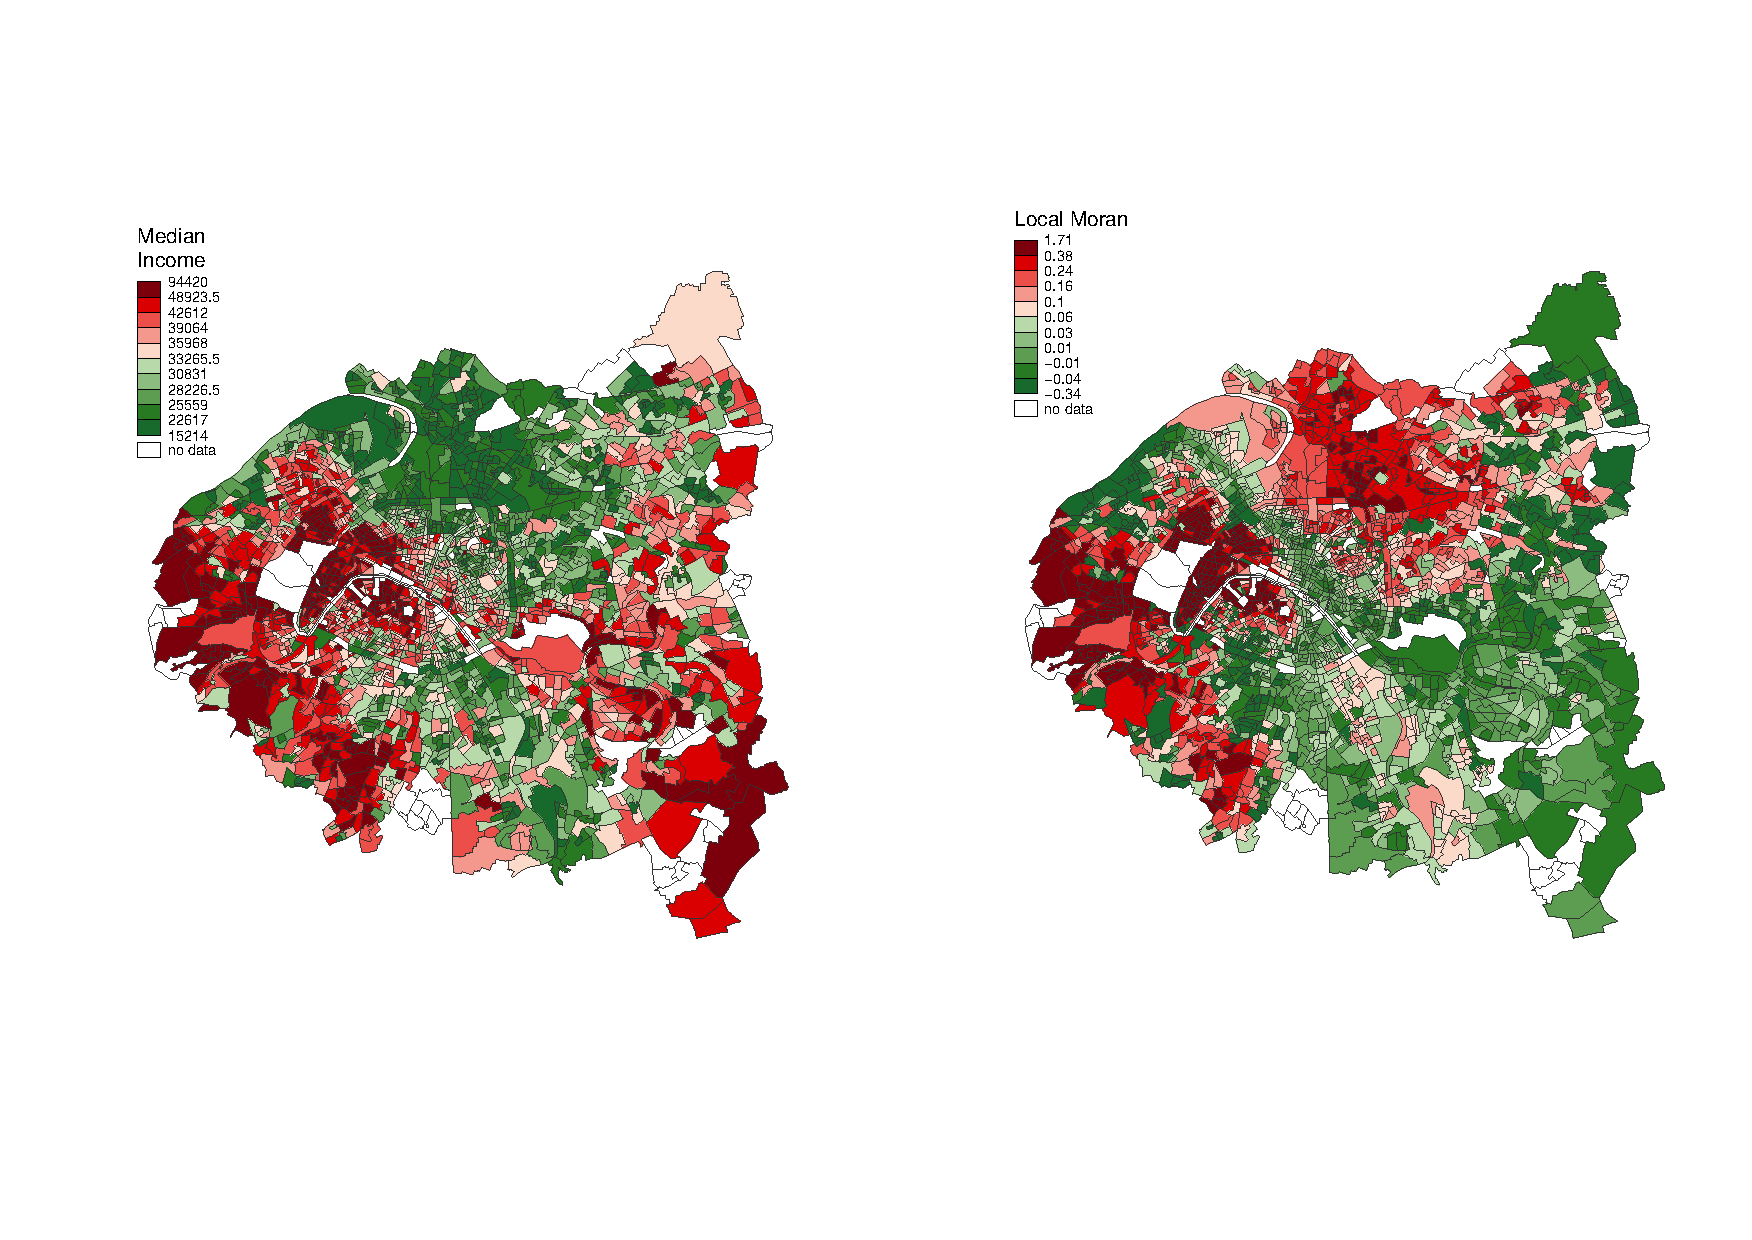
\includegraphics[width=\textwidth]{figures/rob_grandParis_income_moran}

\column{0.35\textwidth}
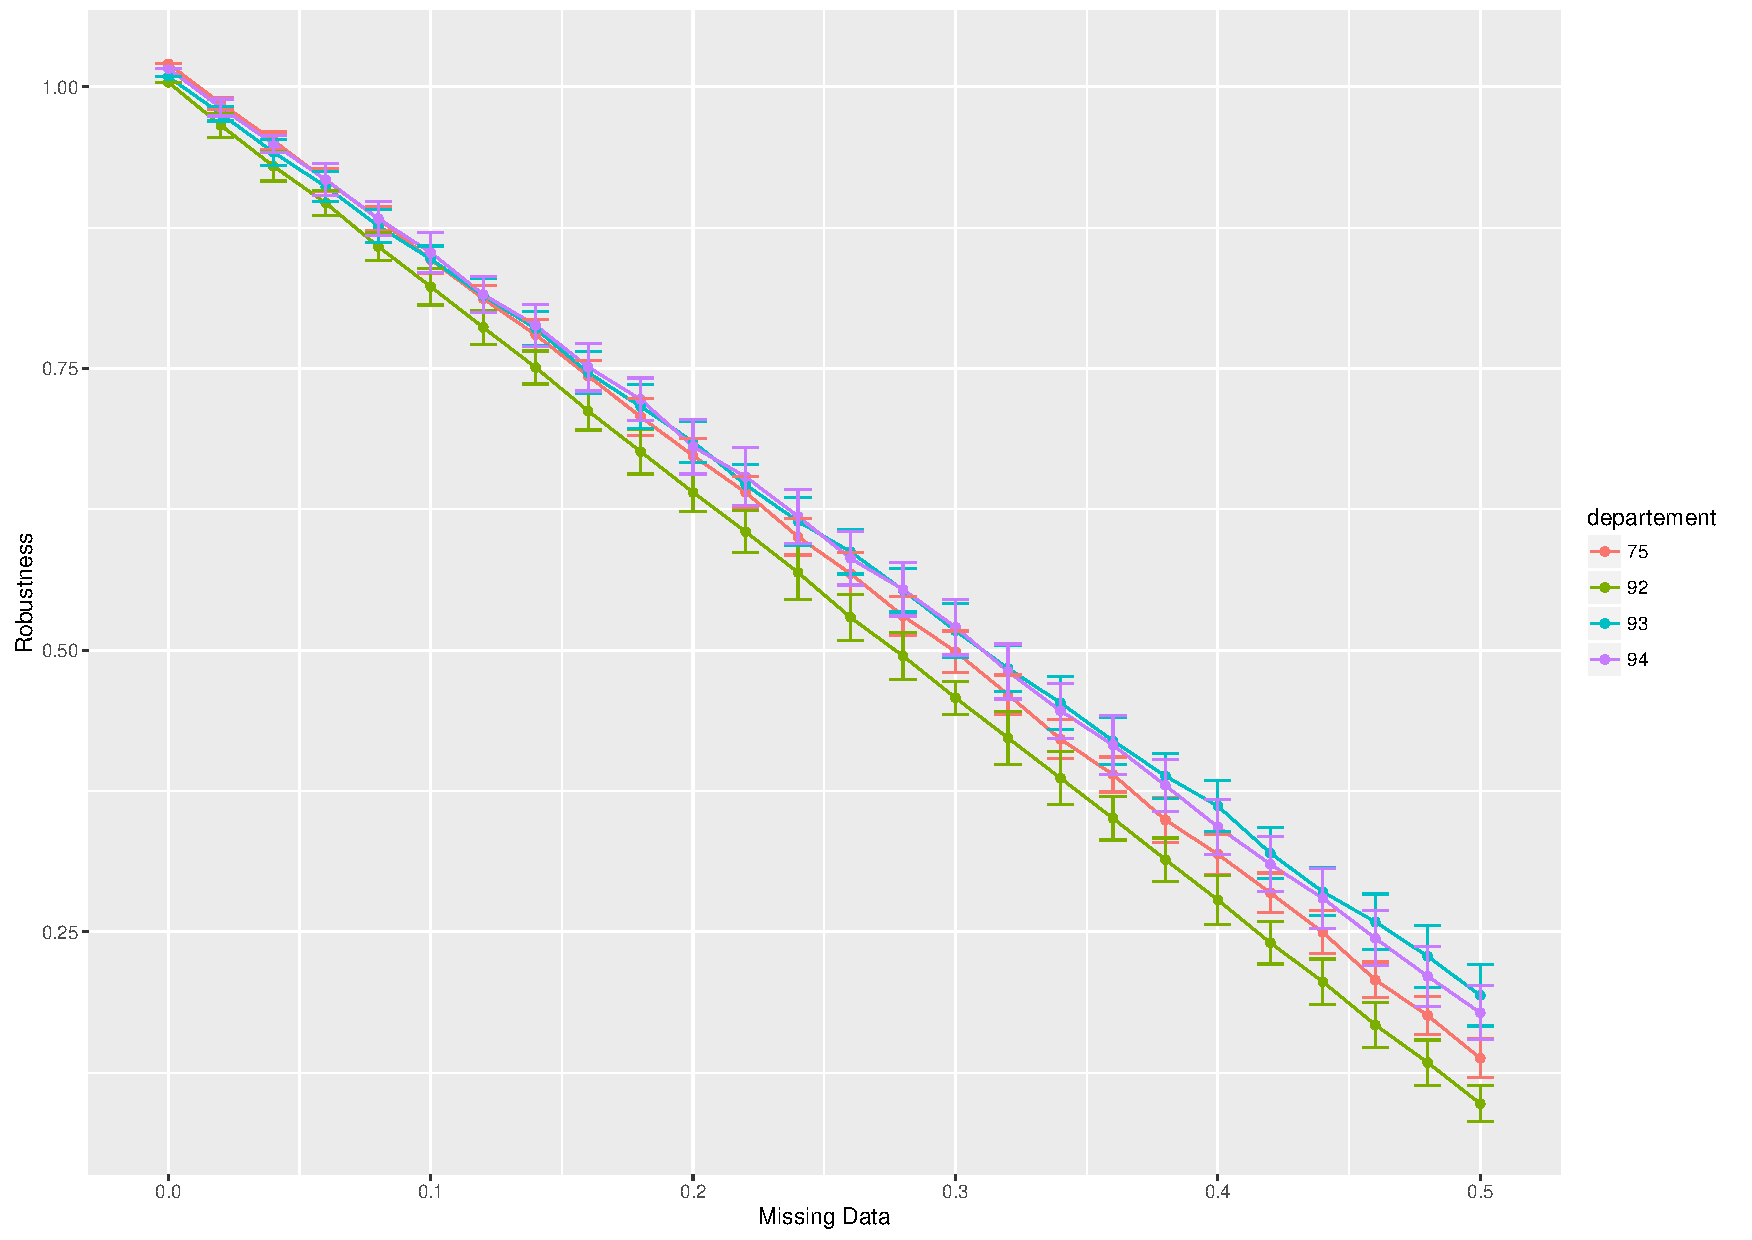
\includegraphics[width=0.7\textwidth]{figures/rob_alldeps_rob_renormindics}\\
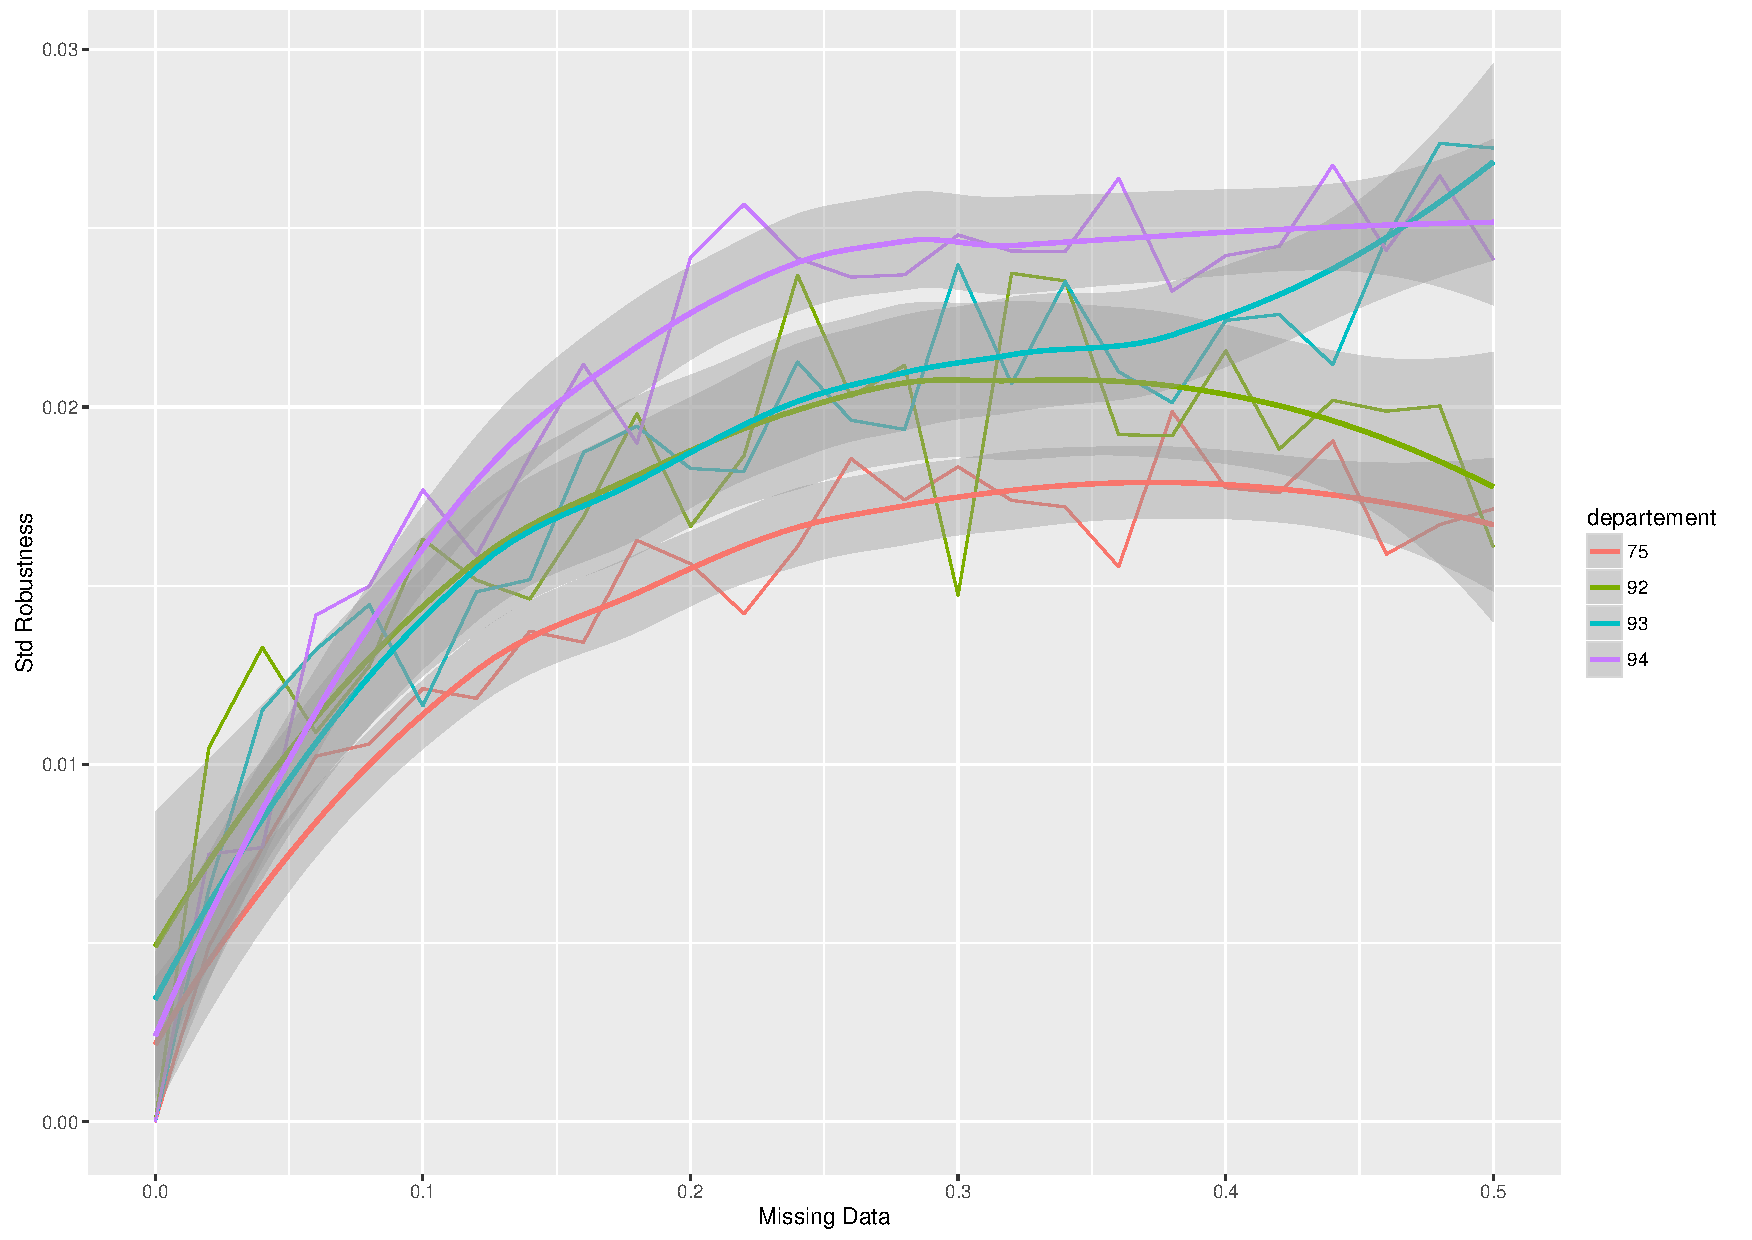
\includegraphics[width=0.7\textwidth]{figures/rob_alldeps_robsd_renormindics}


\end{columns}

}






%%%%%%%%%%%%%%%%%%%%%
\begin{frame}[allowframebreaks]
\frametitle{References}
\bibliographystyle{apalike}
\bibliography{/Users/Juste/Documents/ComplexSystems/CityNetwork/Biblio/Bibtex/CityNetwork,biblio,biblio_jig}
\end{frame}
%%%%%%%%%%%%%%%%%%%%%%%%%%%%









\end{document}







